%# -*- coding: utf-8 -*-
%!TEX encoding = UTF-8 Unicode
%%%%%%%%%%%%%%%%%%%%%%%%%%%%%%%%%%%%%%%%%%%%%%%%%%%%%%%%%%%%%%%%%%%%%%%%%%%%%%%%%%
%论文模板                                                                        %
%此为中文XeLatex-article                                                         %
%                             !编译方式是:XeLaTeX  !                          %
%%%%%%%%%%%%%%%%%%%%%%%%%%%%%%%%%%%%%%%%%%%%%%%%%%%%%%%%%%%%%%%%%%%%%%%%%%%%%%%%%%
\documentclass[12pt]{article}
\usepackage[slantfont,boldfont]{xeCJK}% 允许斜体和粗体
\setCJKmainfont{FangSong}             % 设置缺省中文字体
\setmainfont{Times New Roman}         % 设置Times New Roman为默认的英文字体
\setlength{\parindent}{2.5em}         % 中文缩进两个汉字位

\usepackage{titlesec}%章节标题格式设置
\usepackage{titletoc}%目录格式设置
\usepackage{amsmath}%公式环境数学命令
\usepackage{array}%数组和表格制作
\usepackage[a4paper,top=2.5cm,bottom=2.5cm,left=3cm,right=2cm]{geometry}%版面尺寸设置
\usepackage{multirow}
\usepackage{enumerate}
\usepackage{verbatim,listings}
\usepackage{color}
\usepackage{graphicx}
\usepackage{slashbox}
\usepackage{fancybox}
\usepackage{fancyhdr}
\usepackage{float}    % for fig.pos='H'
\usepackage{rotfloat} % for sidewaysfigure
\usepackage{subfig}   % for subfigure
\usepackage{caption}
\usepackage{subfloat}
%%%%%%%%%%%%%%%%%%%%%%%%%%%%%%%%%%%%%%%%%%%%%%%%%%%%%%%%%%%%%%%%%%%%%%%%%%%%%%%%%%%%%%%%%%%%%%%%%%%%%
%自定义命令:
\makeatletter
%字号设置
\newcommand{\chuhao}{\fontsize{42pt}{\baselineskip}\selectfont}%初号
\newcommand{\xiaochuhao}{\fontsize{36pt}{\baselineskip}\selectfont}%小初号
\newcommand{\yihao}{\fontsize{28pt}{\baselineskip}\selectfont}%一号
\newcommand{\erhao}{\fontsize{21pt}{\baselineskip}\selectfont}%二号
\newcommand{\xiaoerhao}{\fontsize{18pt}{\baselineskip}\selectfont}%小二号
\newcommand{\sanhao}{\fontsize{15.75pt}{\baselineskip}\selectfont}%三号
\newcommand{\xiaosanhao}{\fontsize{15pt}{\baselineskip}\selectfont}%小三号
\newcommand{\sihao}{\fontsize{14pt}{\baselineskip}\selectfont}%四号
\newcommand{\xiaosihao}{\fontsize{12pt}{\baselineskip}\selectfont}%小四号
\newcommand{\wuhao}{\fontsize{10.5pt}{\baselineskip}\selectfont}%五号
\newcommand{\xiaowuhao}{\fontsize{9pt}{\baselineskip}\selectfont}%小五号
\newcommand{\liuhao}{\fontsize{7.875pt}{\baselineskip}\selectfont}%六号
\newcommand{\qihao}{\fontsize{5.25pt}{\baselineskip}\selectfont}%七号

%行间距设置
\renewcommand\baselinestretch{1.25}%1.25倍行距

%页眉页脚设置1
\fancypagestyle{plain}
{
\fancyhead{}
\fancyhead[C]{\wuhao{基于机器学习的信用卡评分模型}}
\fancyfoot{}
\fancyfoot[C]{\thepage}
}
%页眉页脚设置2
\pagestyle{fancy}
{
 \fancyhead{}
 \fancyhead[C]{\wuhao{基于机器学习的信用卡评分模型}}
 \fancyfoot{}
}

%重新定义
\renewcommand\refname{参考文献}
\renewcommand\figurename{图}
\renewcommand\tablename{表}

%表格设置
\newsavebox{\tablebox}


\makeatother
%%%%%%%%%%%%%%%%%%%%%%%%%%%%%%%%%%%%%%%%%%%%%%%%%%%%%%%%%%%%%%%%%%%%%%%%%%%%%%%%%%%%%%%%%%%%%%%%%%%%%


\begin{document}

%%%%%%%%%%%%%%%%%%%%%%%%%%%%%%%%%%%%%%%%%%%%%%%%%%%%%%%%%%%%%%%%%%%%%%%%%%%%%%%%%%%%%%%%%%%%%%%%%%%%%%

%%%%%%%%%%%%%%%%%%封面%%%%%%%%%%%%%%%%%%%%%%%%%%%%%%%%%%%%%%%%%%%%%%%%%%%%%%%%%%%%%%%%%%%%%%%%%%%%%%%%%
\thispagestyle{empty}

\begin{center}

\includegraphics[height=0.15\textwidth]{figures/logo.jpg}

\vspace{4cm}

{\yihao\bf{基于机器学习的信用卡评分模型}}
\end{center}

\vspace{4cm}

{\xiaosanhao\bf
\begin{center}
	\makebox[3cm][l]{队~伍~成~员:}\underbar{\makebox[11cm][c]{王雨聪、郭奇、钟禧儿}}
\end{center}
\begin{center}
	\makebox[3cm][l]{队~伍~名~称:}\underbar{\makebox[11cm][c]{你~说~的~都~队}}
\end{center}

\begin{center}
	\makebox[3cm][l]{专~~~~~~~~~业:}\underbar{\makebox[11cm][c]{大数据分析$\&$应用统计学}}
\end{center}
\begin{center}
	\makebox[3cm][l]{联~系~方~式:}\underbar{\makebox[11cm][c]{Tel:18629537461$\&$13543001390}}
\end{center}
}

\vspace{4cm}


\begin{center}\wuhao\bf
{


\makebox[5cm][c]{二〇二〇年十月}
}
\end{center}

%%%%%%%%%%%%%%%%%%%%%%%%以下命令生成中文摘要%%%%%%%%%%%%%%%%%%%%%%%%%%%%%%%%%%%%%%%%
\newpage
\thispagestyle{fancy}

\begin{center}
%{\sanhao\textbf{摘要上面的题目}}
\end{center}

\renewcommand\abstractname{\xiaosanhao\textbf{摘~~~要}}

\begin{abstract}
\begin{flushleft}
	%\noindent\qquad 表示中文摘要每段断首缩进两个汉字位
	\noindent\qquad 改革开放以来,我国国民经济开始迅猛增长,金融机构与商业银行的信贷等传统信贷产业得到了飞速的发展。
	在传统的商业银行以及资信机构的贷款过程中,通常以实地调查以及资产的抵押来进行对借款人的偿还能力进行分析评估,这种方式不仅效率低,速度慢,在此情况下,如何找到一套可以提高升金融风险识别能力,增强风险评估的准确性,减少人力成本以提高风险管理效率、提高网络借贷的成功率的信用评分系统,是我国金融行业的核心工作之一。\\
	
	\noindent\qquad 在银行与P2P借贷中,评分卡是风险评估的重要工具,能够对借贷申请人进行信用评估打分,预测申请人未来的偿还表现并进行排序。本文以2014年德国某银行的真实数据为基础,首先进行数据初步清洗,筛选重复值,随机森林方法填补缺失值,观察数据分布并去除异常值。特征工程中,对于不平衡的数据,首先使用SMOTE采样方法对样本做平衡化处理,而后绘画每个特征IV曲线筛查有效特征,VIF检验和皮尔逊检验筛选出共线性特征,而后对数据进行卡方分箱处理,分箱后,对数据进行WOE编码。\\
	
	\noindent\qquad 在模型选择上,我们初步使用KNN、SVM和logisitic模型分别进行拟合,并用学习曲线评价不同模型的拟合能力,最后选择logistic模型,而在选定模型后,我们以ROC曲线的面积-AUC的大小作为模型性能评估标准,对其调整参数,使其最优,而后根据信用分模型和评分卡模型,最终制作出评分卡。
	
	
	\vspace{1cm}
	%此处的关键词之间用空格“\quad”隔开
	%一般设置3—8个关键词
	\noindent\textbf{关键词:}评分卡\quad 逻辑回归\quad 机器学习\quad ROC曲线\quad WOE编码\quad
\end{flushleft}
\end{abstract}



%%%%%%%%%%%%%%%%%%%目录%%%%%%%%%%%%%%%%%%%%%%%%%%%%%%%%%%%%%%%%%%%%%%%%%%%%%%%%%%%%%%%%%%%%%%%%%%%%%
\newpage

\thispagestyle{fancy}

\vspace*{1mm}%垂直距离


\renewcommand\contentsname{\xiaosanhao\textbf{目~~~录}}


\tableofcontents

%%%%%%%%%%%%%%%%%%%正文:第1部分%%%%%%%%%%%%%%%%%%%%%%%%%%%%%%%%%%%%%%%%%%%%%%%%%%%%%%%%%%%%%%%%%%%%%
\newpage%新的一页
\pagestyle{plain}
\pagenumbering{arabic}

\section{项目背景及流程}


\begin{flushleft}
	\noindent\qquad 评分卡是一个贷前评分体系,用于对未来一段时间内借贷申请人违约、逾期、失联概率的预测,分数越高表示该客户借贷风险越低,反之如果分数较低,表示对该客户的借贷风险较高,银行和资信机构可以拒绝该申请者的贷款业务。\\
	\noindent\qquad 在以往的传统金融学分析中,银行等贷款机构主要采用专家赋值的办法产生供业务人员使用的评分卡,往往由于信息不对等或者决策者的主观意识而造成一部分贷款申请客户难以通过贷款申请。\\
	\noindent\qquad 不过在当代,金融机构在风险管理的每个环节都尽可能地引入统计学计量分析的方法,依托大数据进行后台的分析回顾,不断的优化调整,使得金融机构在风险与收益的博弈过程中更快达到平衡。\\
	\noindent\qquad 我们将以2014年德国某银行的真实数据为基础,制作评分卡,评分卡制作出来后,可以对银行中的每一个客户进行打分,客户分的高低,成为衡量客户信用、银行对客户借贷成功率判断的辅助手段,以下为评分卡制作的流程,大图可于附件中查看。
\end{flushleft}






\begin{figure}[H]
	\centering
	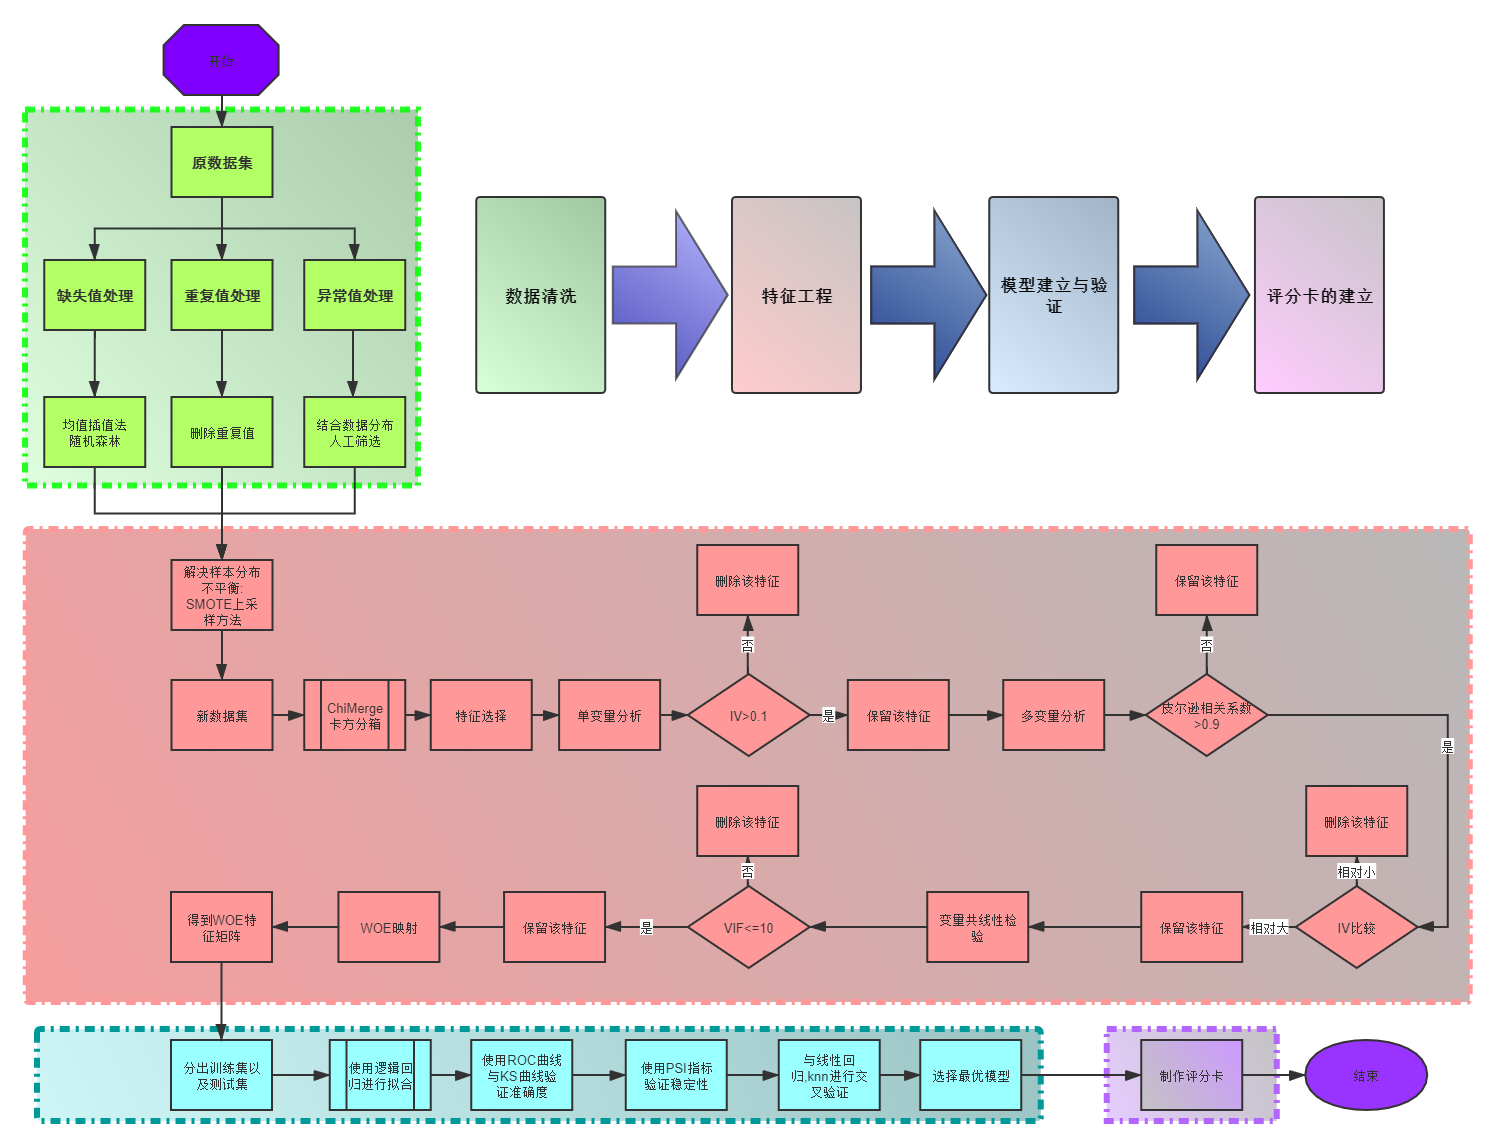
\includegraphics[width=1\linewidth]{figures/思维导图2.0}
	\caption{}
	
\end{figure}

\newpage
\section{数据清洗}

\subsection{数据来源及数据特征信息}
本文使用的数据集来自于竞赛网站Kaggle,名字叫做GivemeSomeCredit,源自2014年一家德国银行的真实数据。经观察,该数据集总共10个特征值,1个标签值,如图所示:

\vspace{2cm}

\begin{tabular}{|c|c|}
	\hline 
	SeriousDlqin2yrs & 好客户与坏客户 \\ 
	\hline 
	RevolvingUtilizationOfUnsecuredLines & 无担保贷款的循环利用 \\ 
	\hline 
	age  & 借款人借款时的年龄 \\ 
	\hline 
	NumberOfTime30-59DaysPastDueNotWorse & 35-59天逾期但不糟糕次数 \\ 
	\hline 
	DebtRatio  & 负债比率 \\ 
	\hline 
	MonthlyIncome & 月收入 \\ 
	\hline 
	NumberOfOpenCreditLinesAndLoans & 开放式信贷和贷款数量 \\ 
	\hline 
	NumberOfTimes90DaysLate & 90天逾期次数 \\ 
	\hline 
	NumberRealEstateLoansOrLines & 不动产贷款或额度数量 \\ 
	\hline 
	NumberOfTime60-89DaysPastDueNotWorse  & 60-89天逾期但不糟糕次数 \\ 
	\hline 
	NumberOfDependents  & 家属数量 \\ 
	\hline 
\end{tabular} 
\begin{center}
	表(1)
\end{center}
\vspace{2cm}

由于特征值较多,不便于观察与后续分析。我们依照不同属性把十个特征值进行适当的分类。这些特征经过分类,可以归为以下几个属性:
\begin{itemize}
	\item 基本属性:包括了借款人当时的年龄。
	\item 偿债能力:包括了借款人的月收入、负债比率
	\item 信用往来:两年内35-59天逾期次数、两年内60-89天逾期次数、两年内90天或高于90天逾期的次数。
	\item 财产状况:包括了开放式信贷和贷款数量、不动产贷款或额度数量。
	\item 其他因素:包括了借款人的家属数量(不包括本人在内)。
\end{itemize}

\newpage



\subsection{重复值处理}
\subsubsection{处理前与处理后的表格}
\begin{tabular}{|c|c|c|}
	\hline 
	特征名  & 非空值统计  & 数据类型 \\ 
	\hline 
	SeriousDlqin2yrs & 150000 non-null & int64  \\ 
	\hline 
	RevolvingUtilizationOfUnsecuredLines & 150000 non-null & float64 \\ 
	\hline 
	age & 150000 non-null & int64  \\ 
	\hline 
	NumberOfTime30-59DaysPastDueNotWorse & 150000 non-null & int64  \\ 
	\hline 
	DebtRatio   & 150000 non-null & float64 \\ 
	\hline 
	MonthlyIncome & 120269 non-null & float64 \\ 
	\hline 
	NumberOfOpenCreditLinesAndLoans & 150000 non-null & int64 \\ 
	\hline 
	NumberOfTimes90DaysLate  & 150000 non-null & int64 \\ 
	\hline 
	NumberRealEstateLoansOrLines  & 150000 non-null & int64 \\ 
	\hline 
	NumberOfTime60-89DaysPastDueNotWorse & 150000 non-null & int64 \\ 
	\hline 
	NumberOfDependents & 146076 non-null & float64 \\ 
	\hline 
\end{tabular} 
\begin{center}
	表(2)重复值处理前
\end{center}
\vspace{1cm}

\vspace{1cm}

\begin{tabular}{|c|c|c|}
	\hline 
	特征名  & 非空值统计  & 数据类型 \\ 
	\hline 
	SeriousDlqin2yrs & 149391 non-null & int64  \\ 
	\hline 
	RevolvingUtilizationOfUnsecuredLines & 149391 non-null & float64 \\ 
	\hline 
	age & 149391 non-null & int64  \\ 
	\hline 
	NumberOfTime30-59DaysPastDueNotWorse & 149391 non-null & int64  \\ 
	\hline 
	DebtRatio   & 149391 non-null & float64 \\ 
	\hline 
	MonthlyIncome & 120170 non-null & float64 \\ 
	\hline 
	NumberOfOpenCreditLinesAndLoans & 149391 non-null & int64 \\ 
	\hline 
	NumberOfTimes90DaysLate  & 149391 non-null & int64 \\ 
	\hline 
	NumberRealEstateLoansOrLines  & 149391 non-null & int64 \\ 
	\hline 
	NumberOfTime60-89DaysPastDueNotWorse & 149391 non-null & int64 \\ 
	\hline 
	NumberOfDependents & 145563  non-null & float64 \\ 
	\hline 
\end{tabular} 
\begin{center}
	表(3)重复值处理后
\end{center}
\newpage

\subsection{缺失值处理}

\begin{flushleft}
	\noindent\qquad 对于缺失值,我们一般有两种处理方法,一种是直接删除整行的数据,一种是进行填补,从下图我们可以看出数据的缺失情况:
\end{flushleft}

\begin{figure}[H]
	\centering
	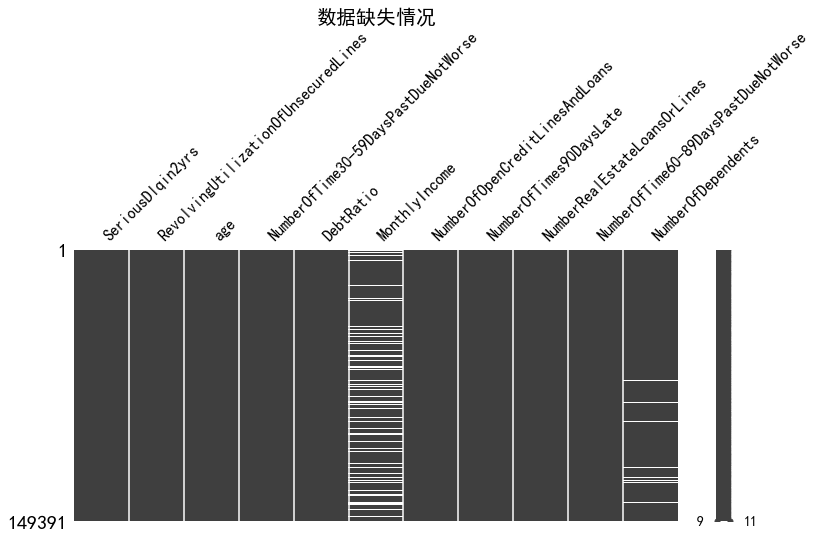
\includegraphics[width=0.8\linewidth]{figures/3}
	\caption{}
\end{figure}

\begin{flushleft}
	\noindent\qquad 白色代表缺失,在这里我们需要填补的特征是“月收入”和“家属人数”,家庭人数的缺失不严重,只占到该特征的百分之二左右,对于“家庭人数”,我们可以直接删去,也可以填充,这里使用均值法进行填充,即取缺失数据周围数据的均值进行填充:
\end{flushleft}

\begin{figure}[H]
	\centering
	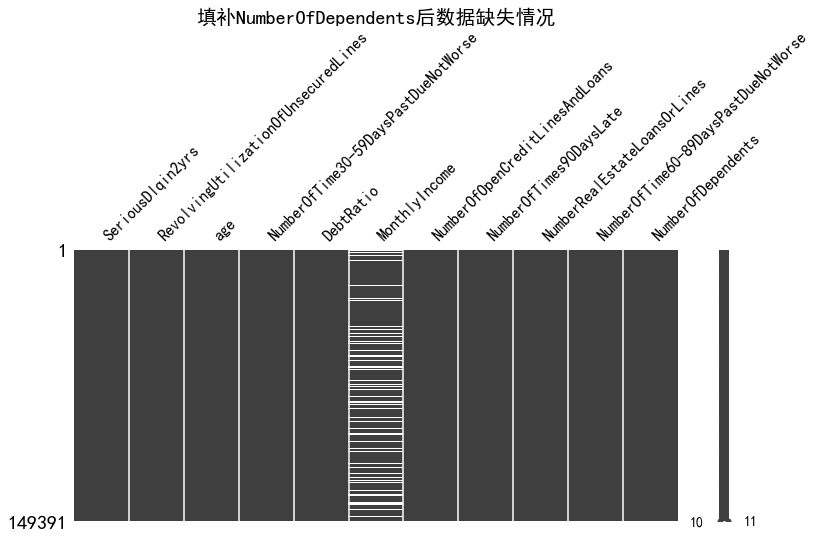
\includegraphics[width=0.8\linewidth]{figures/4}
	\caption{}
\end{figure}

\vspace{1cm}
\begin{flushleft}
	\noindent\qquad “月收入”的缺失比较严重,占到了百分之二十左右,同时,从业务的角度考虑,收入应该是对信用评分来说一个很重要的因素,因此这个特征必须要进行填补,但是均值填补法,对于缺失比例较大的“月收入”,显然是不合适的,我们可以这样去考虑这个问题,一个人来借钱,他应该知道,高收入和稳定收入对于他而言应该是一个有益的证据,因此,如果收入较高或者稳定的客户,他会更加倾向于将自己的收入填上,那么收入栏缺失的客户,更有可能是收入不稳定或者收入比较低的,根据这种判断,我们可以用四分位数来填补缺失值,将收入栏空的客户全部当成低收入人群,当然,这种方法并不严谨,也有可能这种缺失确实是数据收集过程中造成的失误,最好的方法是去和业务人员沟通,观察缺失值是如何产生的。在这里,我们采用随机森林法来进行填充。
\end{flushleft}

\vspace{2cm}

\begin{figure}[H]
	\centering
	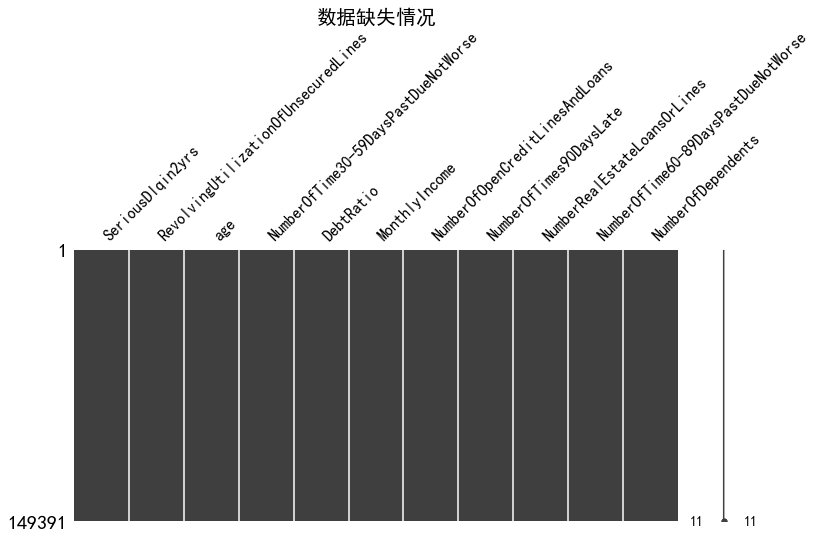
\includegraphics[width=0.9\linewidth]{figures/思维导图中可视化部分/绿色-缺失值处理/3}
	\caption{}
\end{figure}

\newpage
\subsection{异常值处理}
\begin{flushleft}
	\noindent\qquad 在传统的数据分析中,一般要求需要处理的异常值包括极大极小值,离群值,不符合业务逻辑的值,而在银行数据中,我们希望排除的一些异常值并不是一些超高或者超低的值,而是一些不符合业务逻辑,甚至不符合常理的值,在这里我们使用每个特征的核密度估计图来尝试挑出这些异常值,从中可以看出数据的呈现长尾分布,具有高方差的特性,符合我们对银行数据模式的认知
\end{flushleft}
\begin{figure}[H]
	\centering
	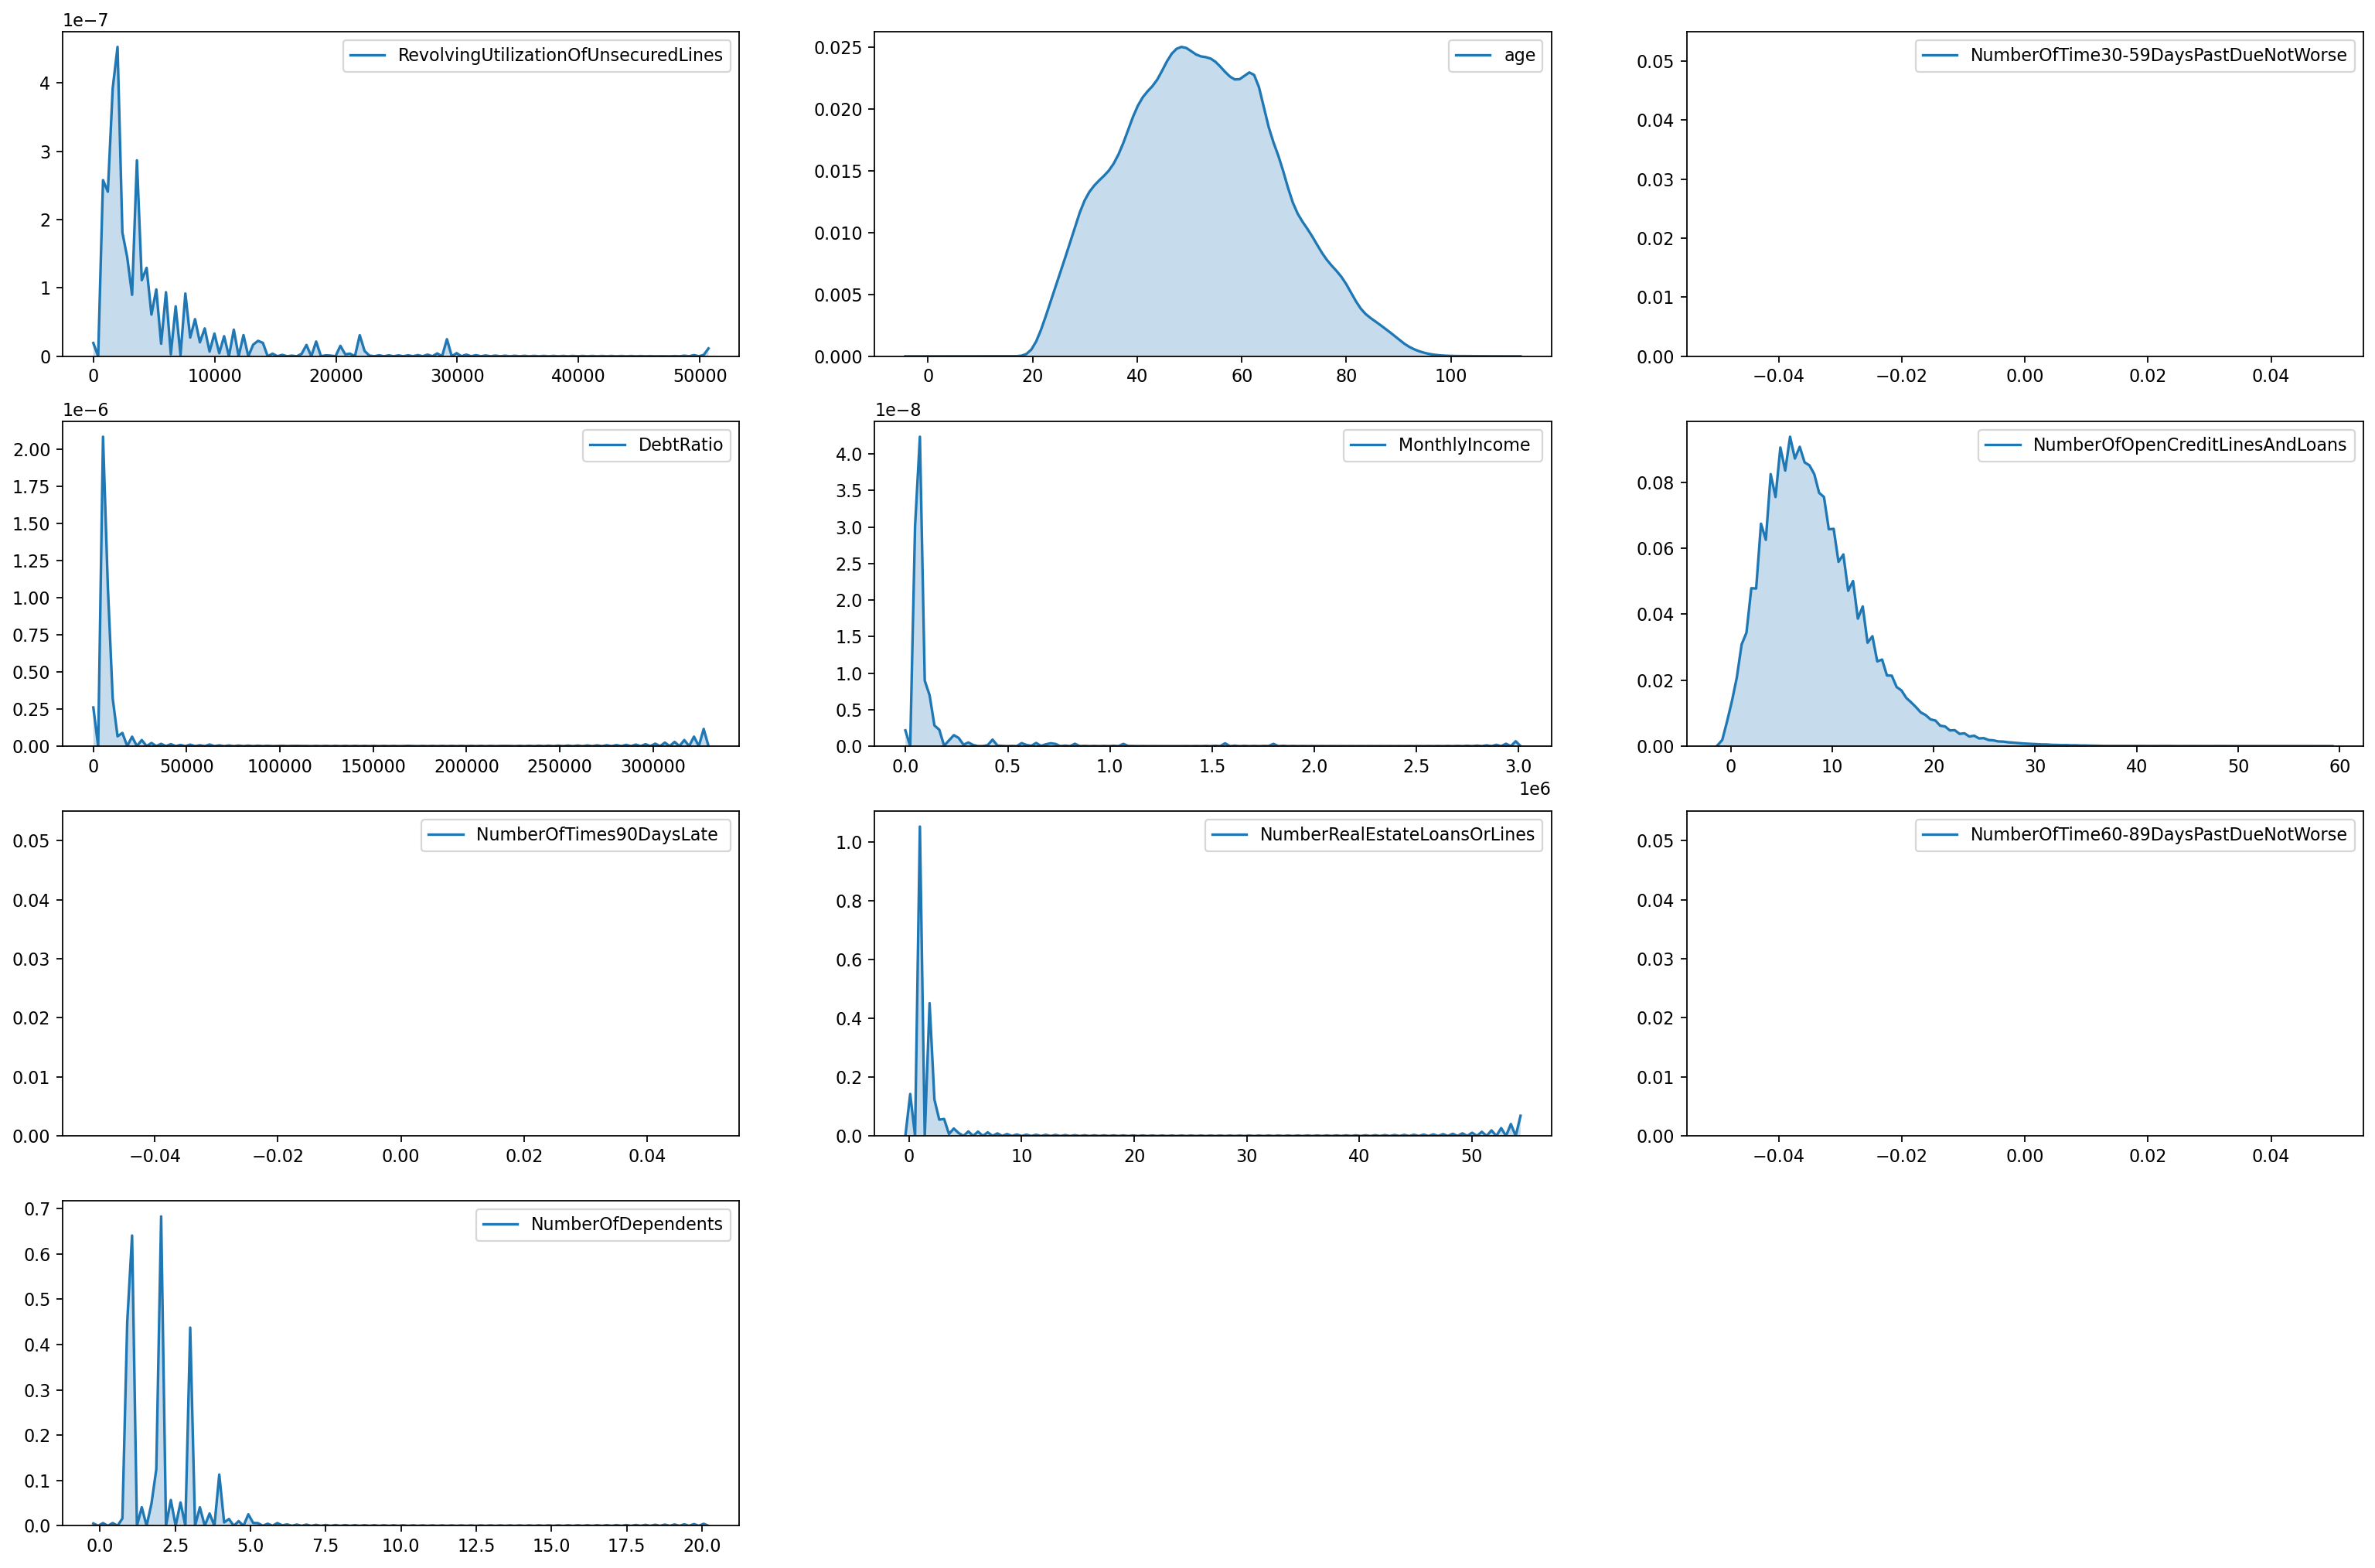
\includegraphics[width=0.7\linewidth]{figures/20201025213636236}
	\caption{}
\end{figure}

\begin{flushleft}
	\noindent\qquad 其中,最小的年龄竟然有0岁,这不符合常理,银行借贷的最小年龄是8岁,经过检查,发现只有一例样本存在这种情况,基本可以确定是异常值,删除即可,另外,有三个指标看起来很奇怪:
	“NumberOfTime30-59DaysPastDueNotWorse”  “NumberOfTime60-89DaysPastDueNotWorse” “NumberOfTimes90DaysLate”\\
		\noindent\qquad 这三个指标分别是:
	“过去两年内出现35-59天逾期但是没有发展的更坏的次数”,
	“过去两年内出现60-89天逾期但是没 有发展的更坏的次数”,
	“过去两年内出现90天逾期的次数”。\\
		\noindent\qquad 这三个指标,在99$\%$的分布的时候依然是2,最大值却是 98,看起来非常奇怪。一个人在过去两年内逾期35~59天98次,一年6个60天,两年内逾期98次这是怎么算出来的? 我们不知道这个指标是如何计算出来的。经过统计发现,在这三个特征中,大于90的值全部属于同一批样本,共225个,所以我们先假设上面三个指标中只要每一项均大于90就将样本认定为异常的。
\end{flushleft}

\newpage




\begin{figure}[H]
	\centering
	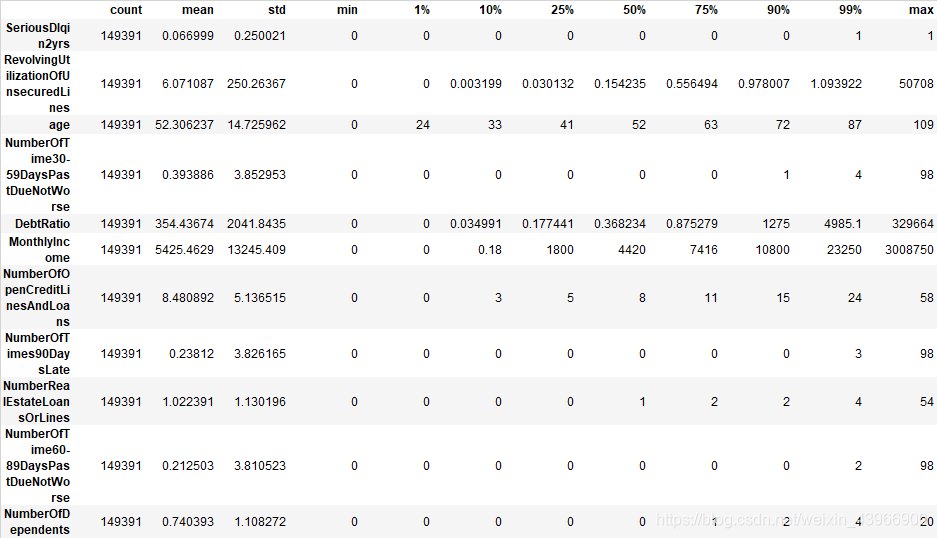
\includegraphics[width=1\linewidth]{figures/sd1}
	\caption{特征的分布,大图请于附件查看}
	
\end{figure}

\begin{figure}[H]
	\centering

	\subfloat[NumberOfTime30-59DaysPastDueNotWorse的分布]{
		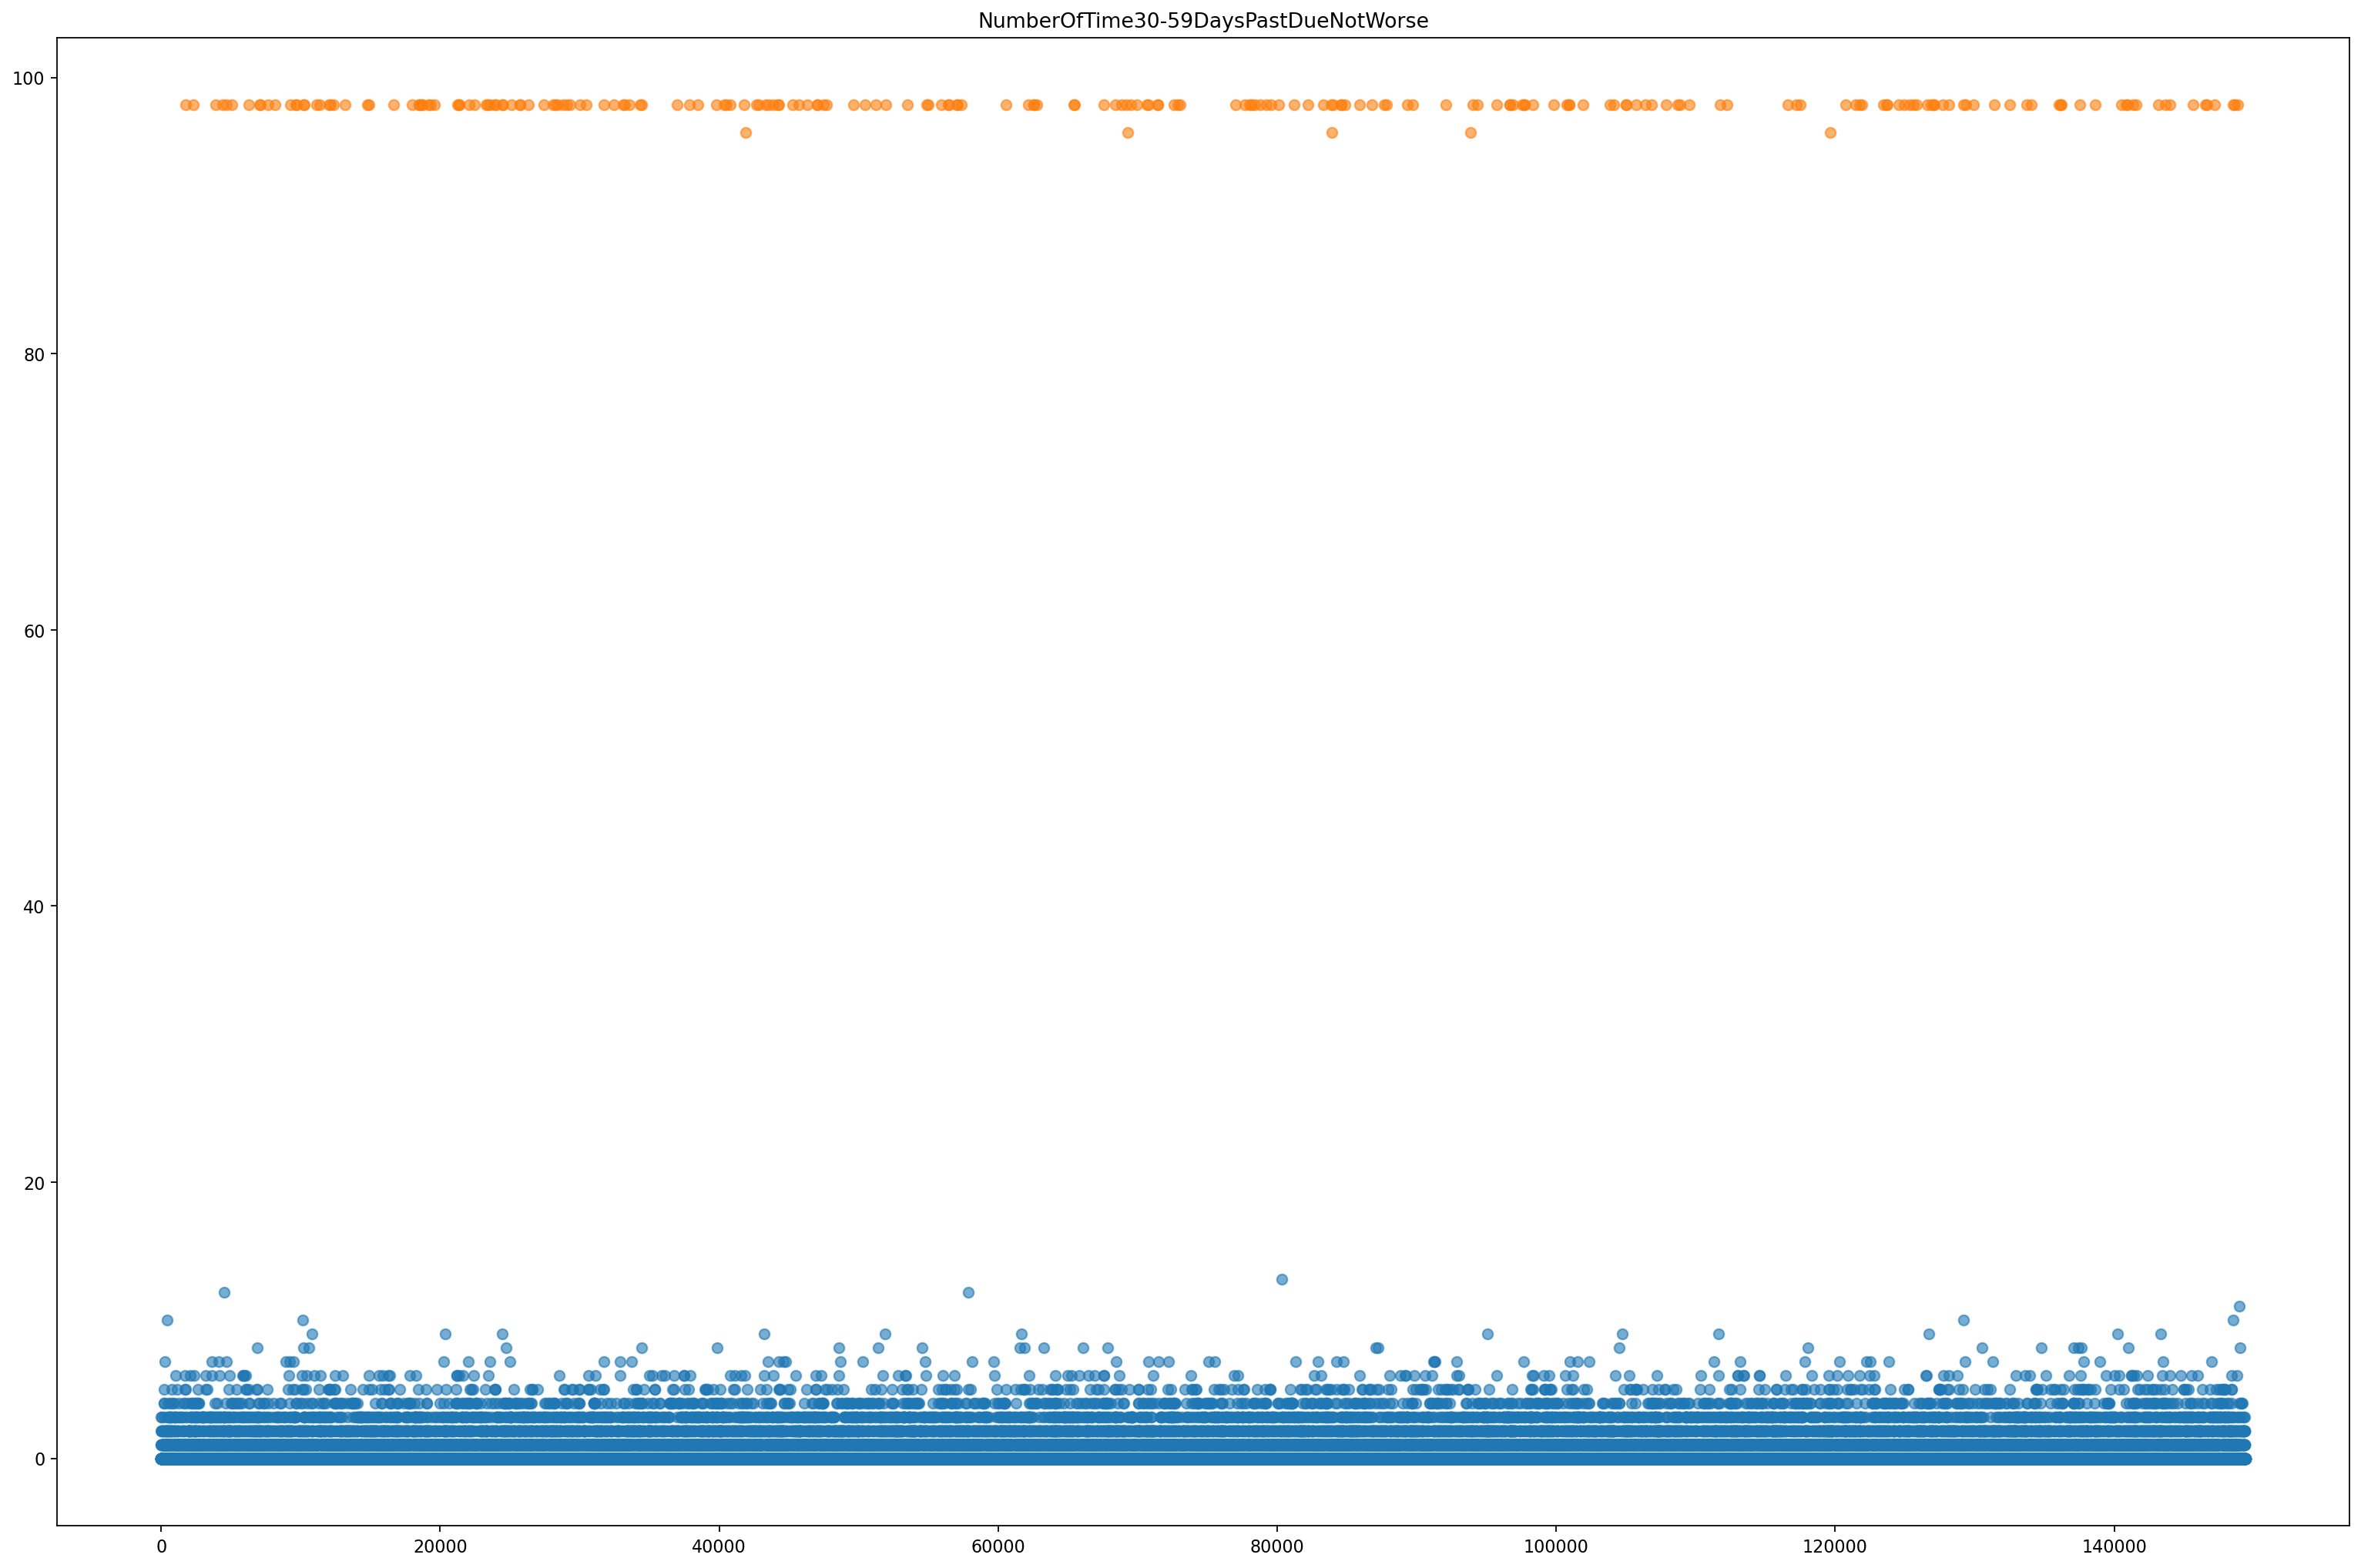
\includegraphics[width=7cm]{figures/plot1}
	}
	\quad
	\subfloat[NumberOfTimes90DaysLate的分布]{
		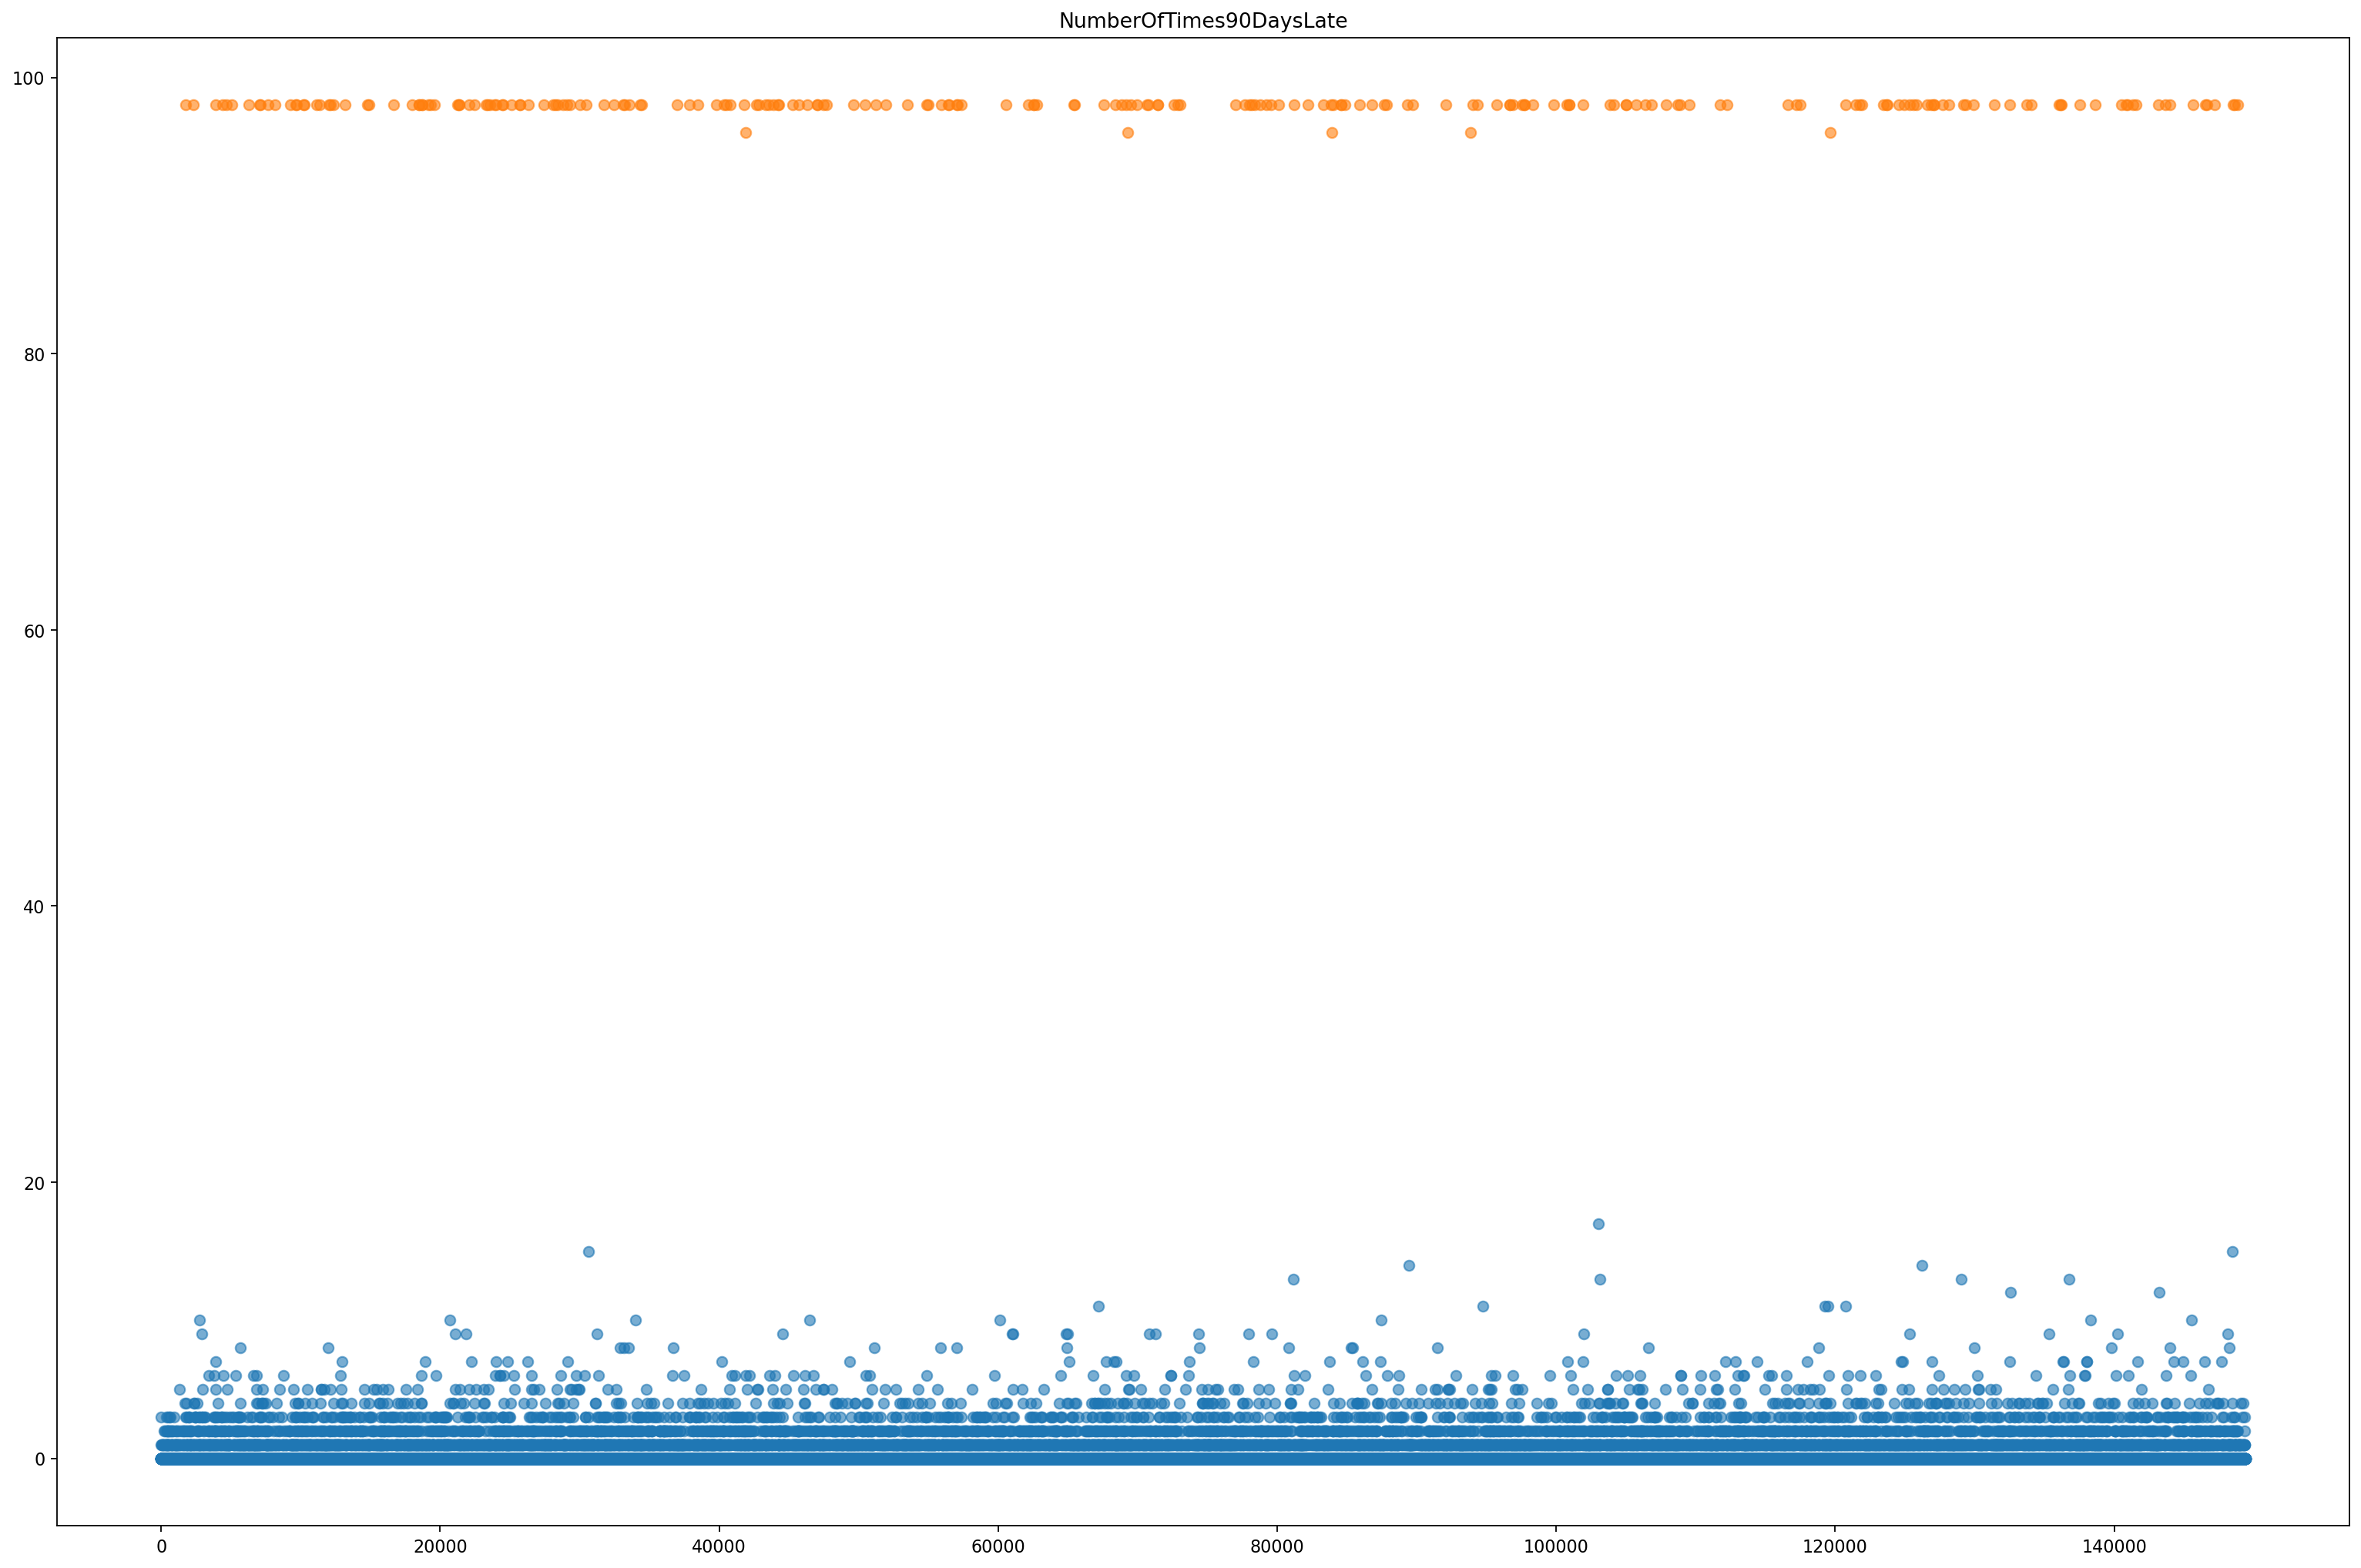
\includegraphics[width=7cm]{figures/plot2}
	}
	\quad
	\subfloat[NumberOfTime60-89DaysPastDueNotWorse的分布]{
		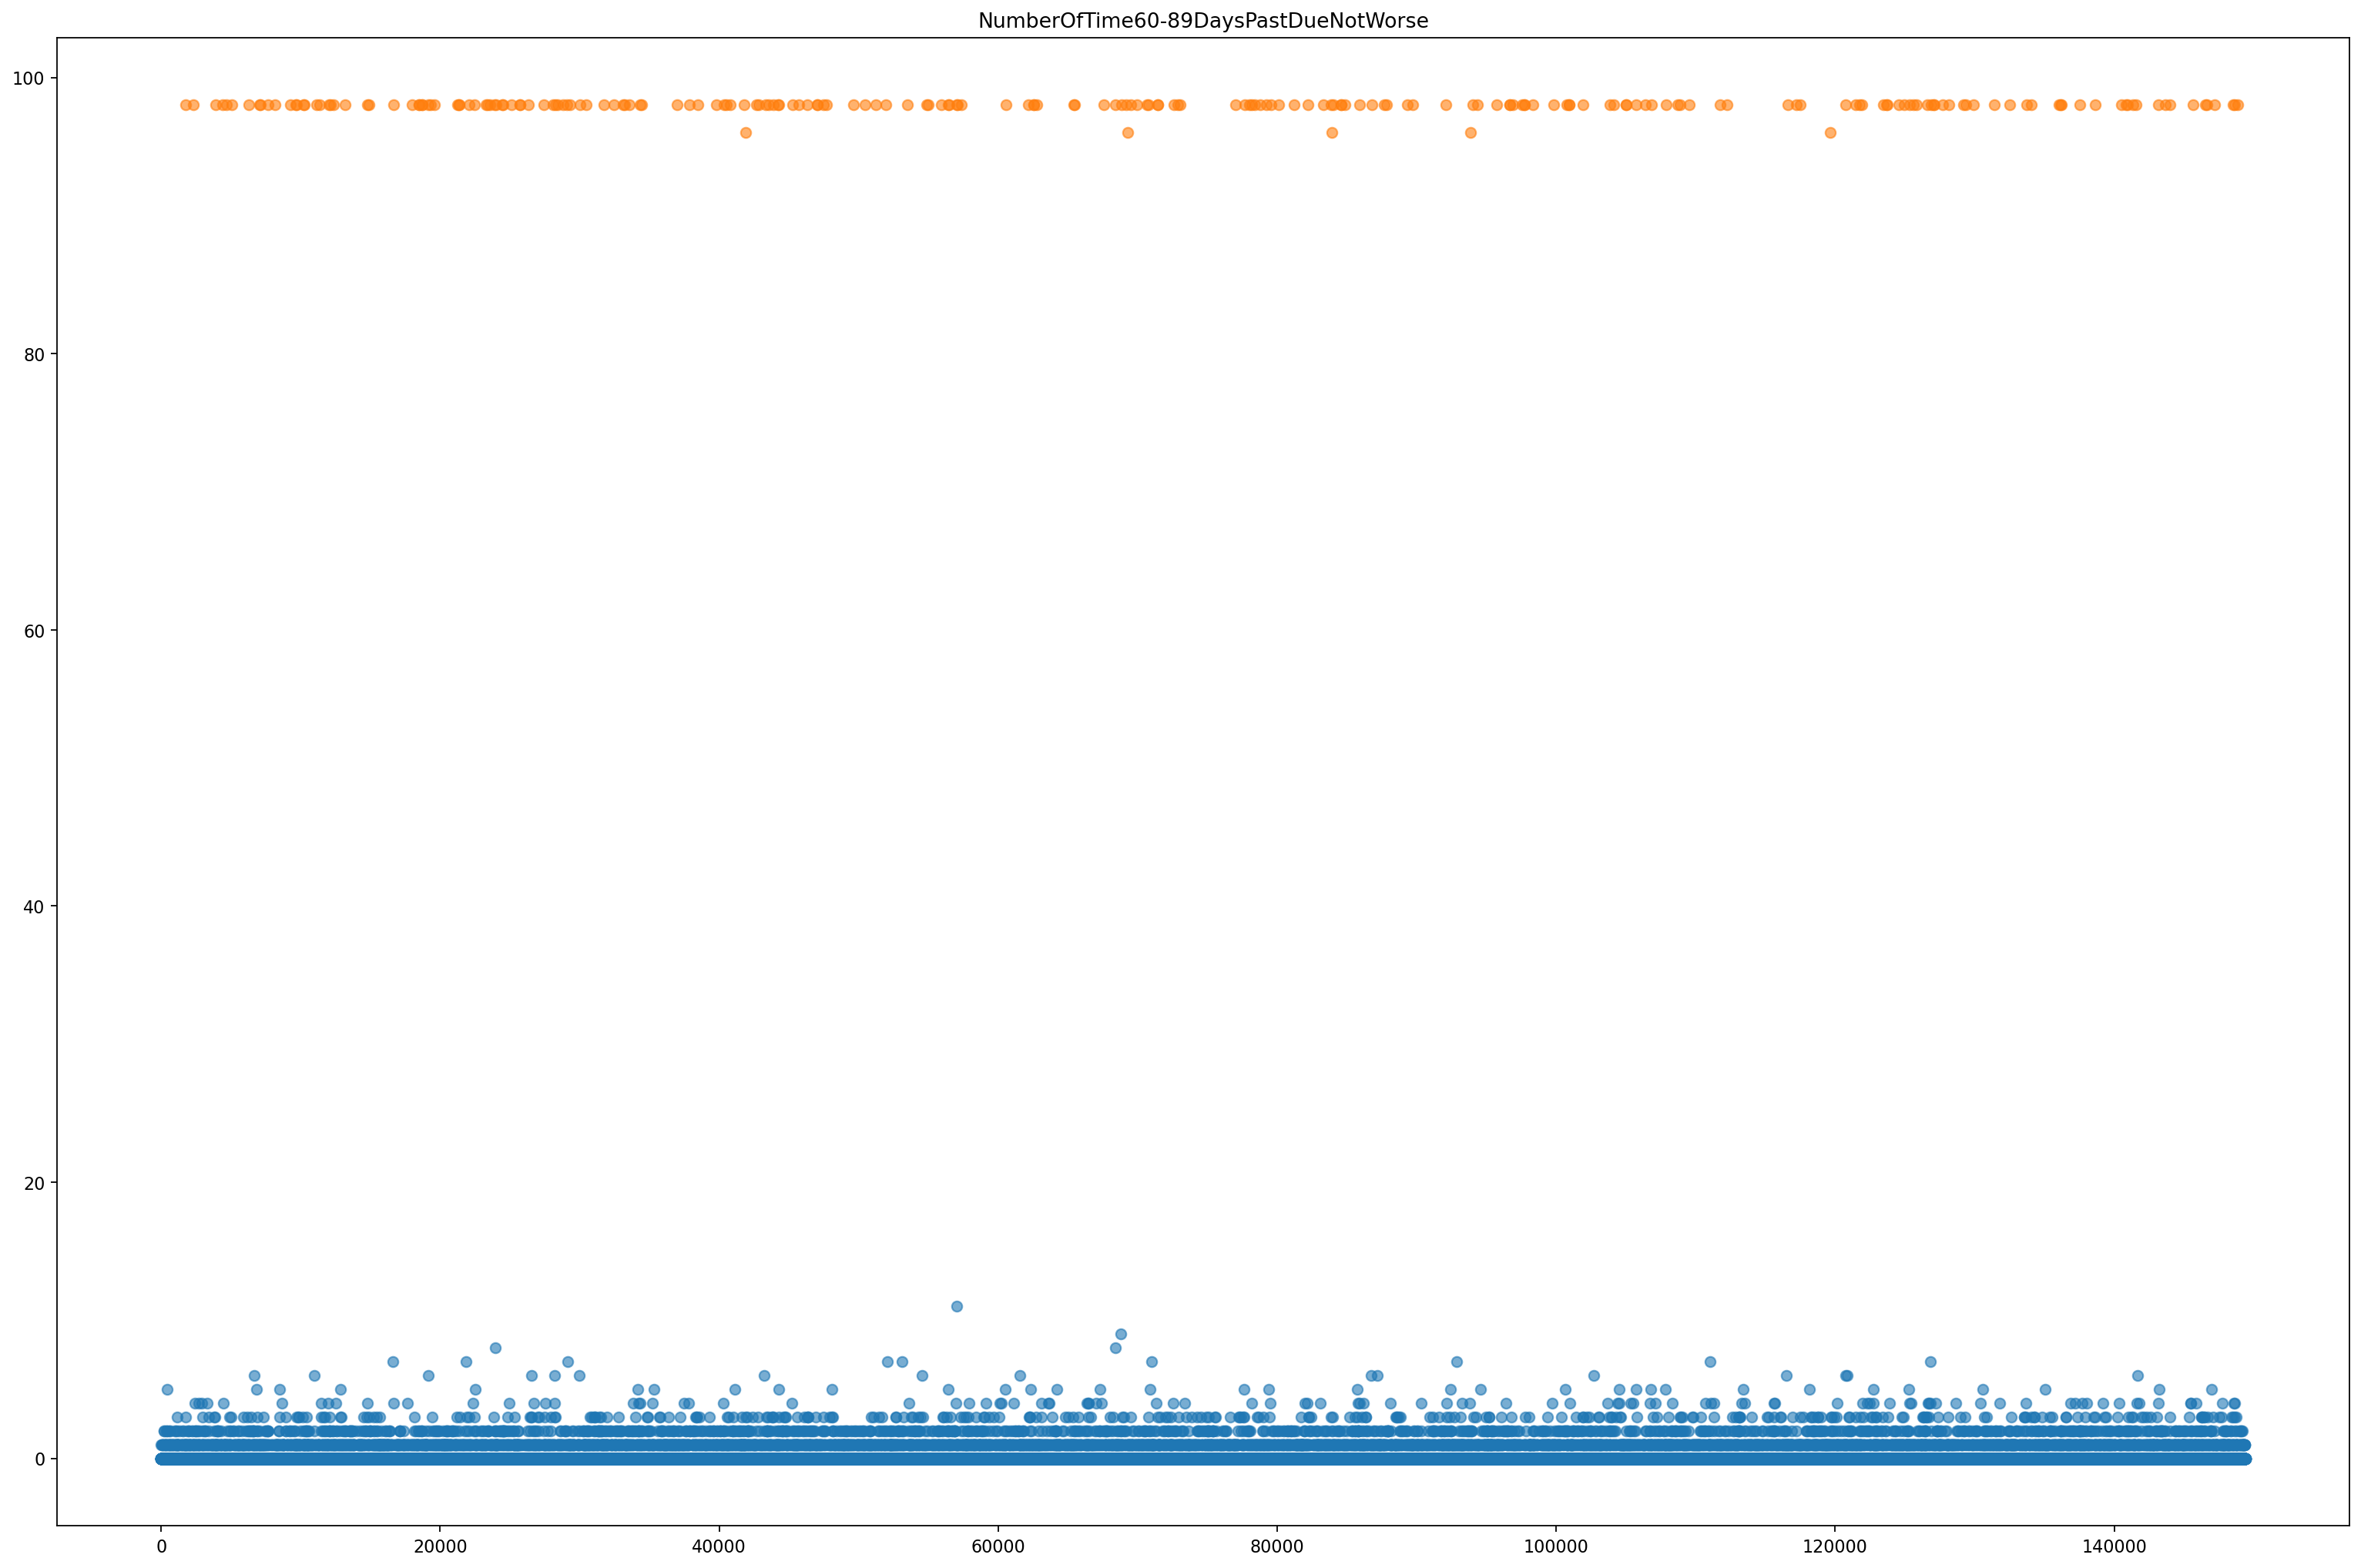
\includegraphics[width=7cm]{figures/plot3}
	}
	\caption{三种特征的分布}
\end{figure}






\newpage
\begin{flushleft}
	\noindent\qquad 那这些两年内逾期了98次的客户,应该都是坏客户。那么通过小提琴图检查是否是这样:
	
\end{flushleft}

\begin{figure}[H]
	\centering
	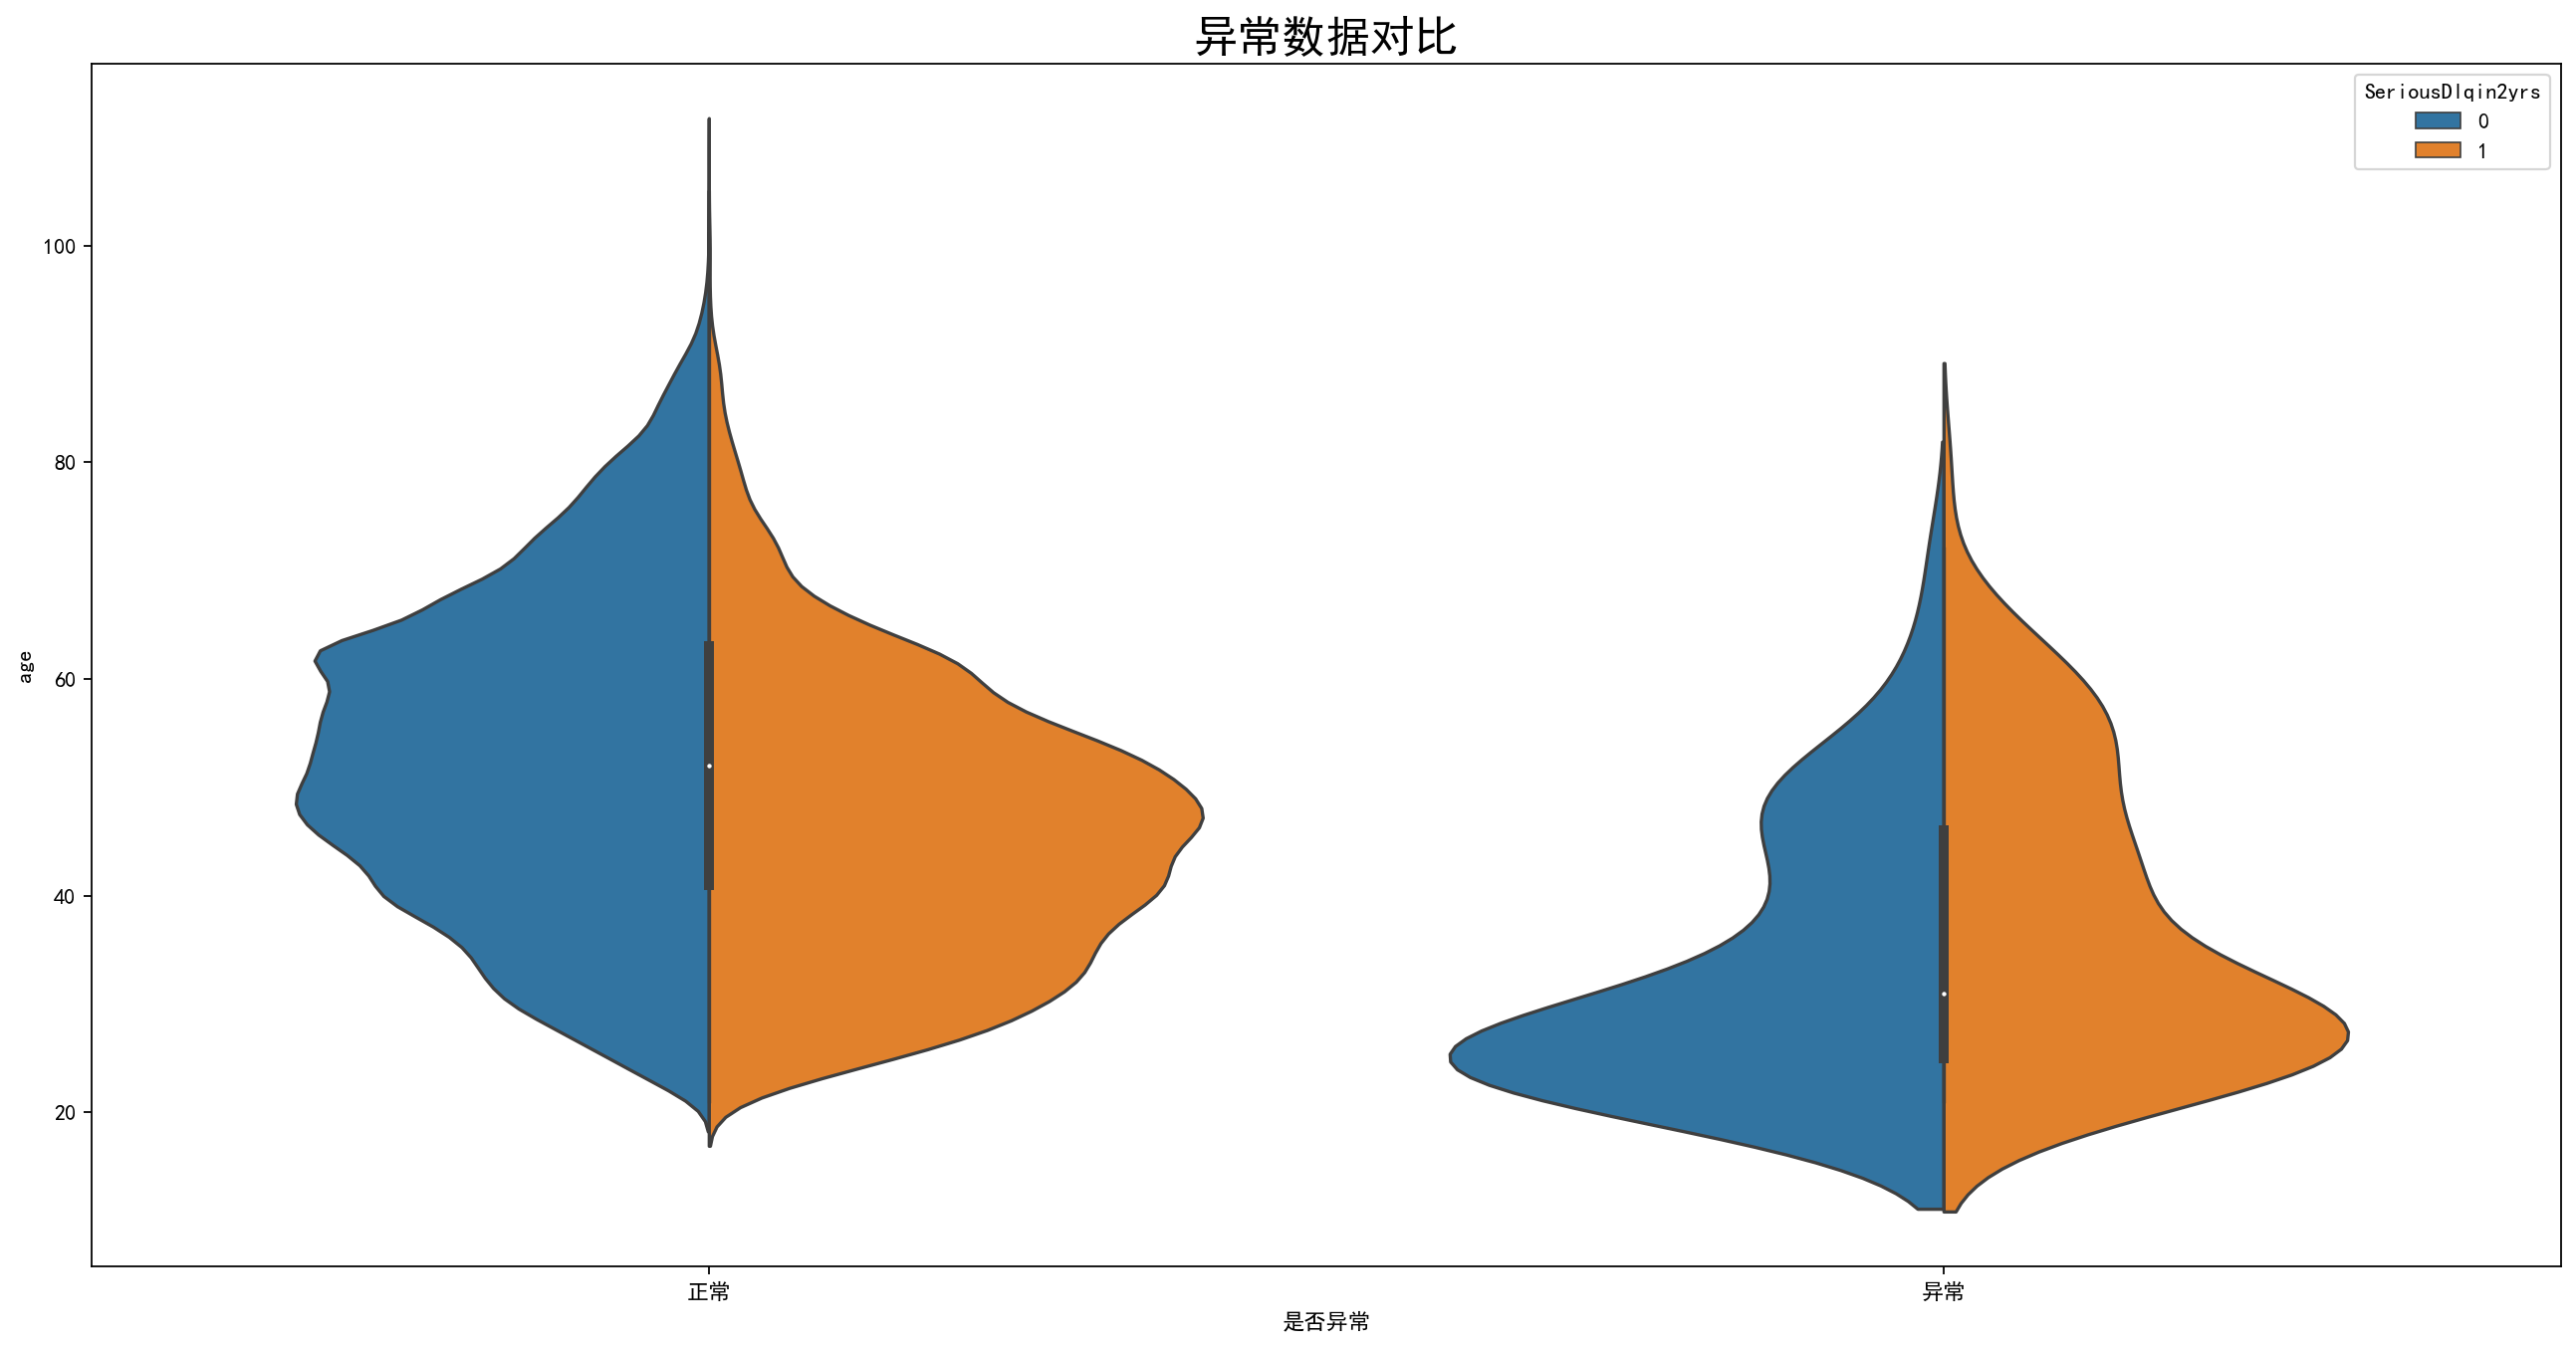
\includegraphics[width=1\linewidth]{figures/plot4}
	\caption{}
\end{figure}

\begin{flushleft}
	\noindent\qquad 可以发现,并不是所有人都违约,但是与正常的数据相比,违约的占多数。同时我们还发现一个很有趣的现象,那就是,这部分异常的数据普遍收入很低。
	
\end{flushleft}

\begin{figure}[H]
	\centering
	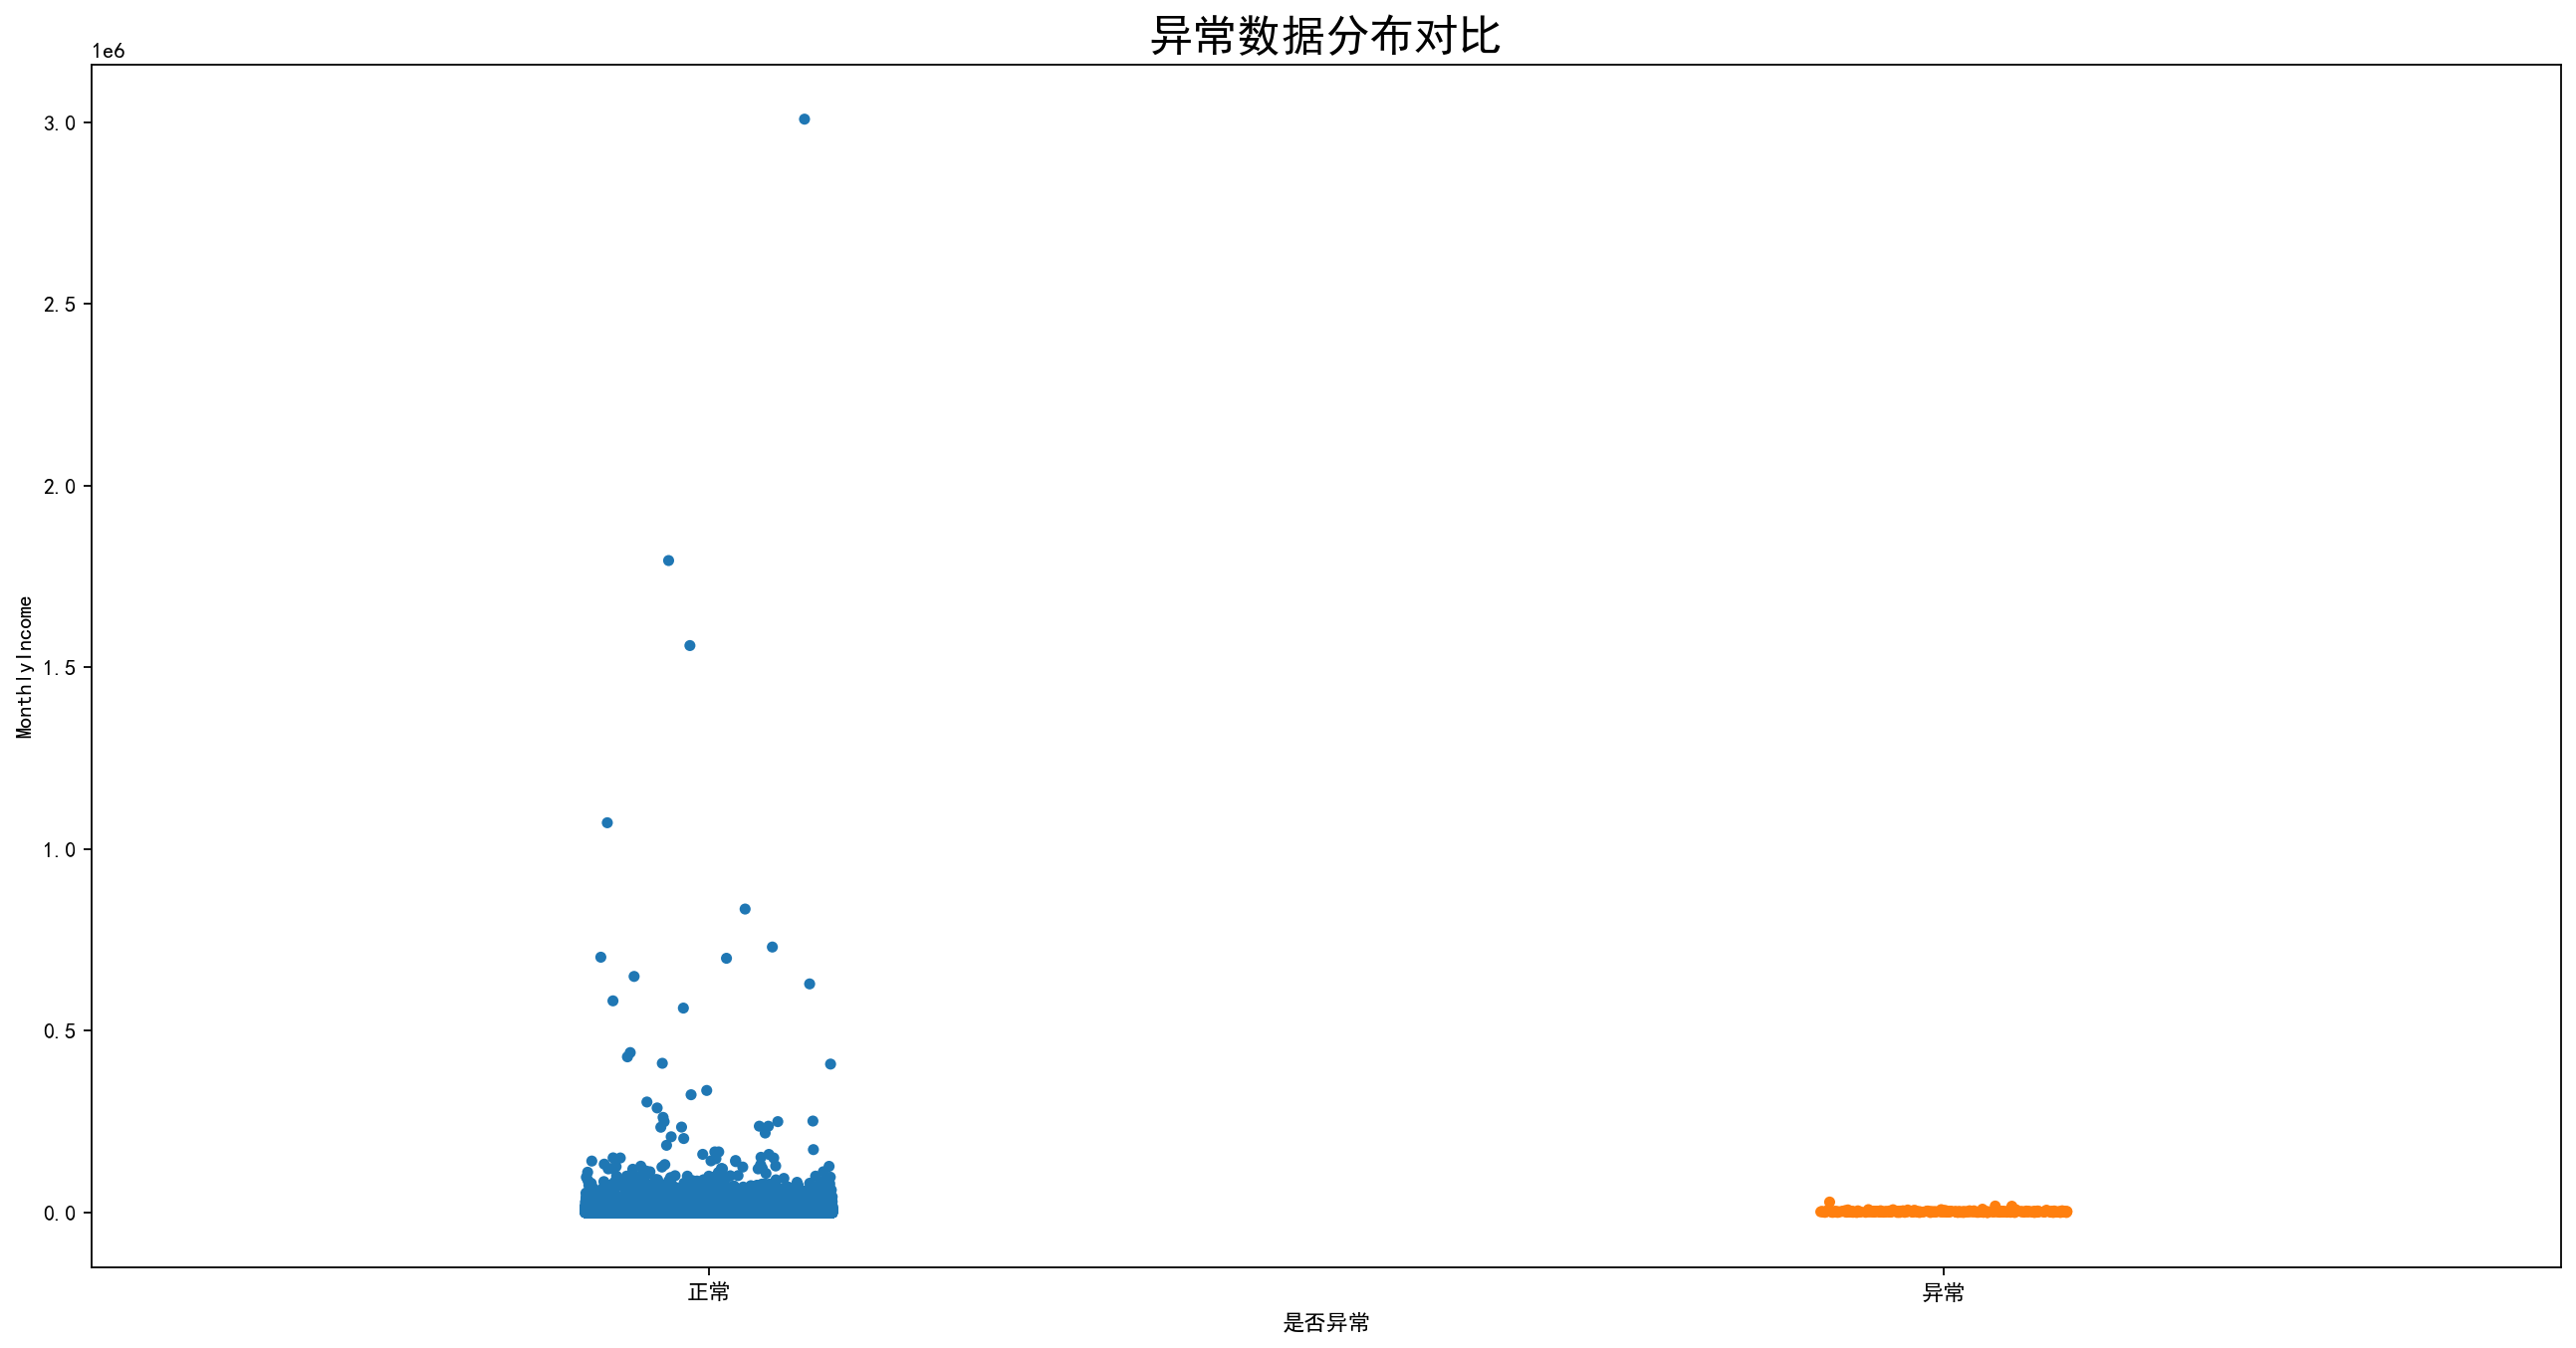
\includegraphics[width=1\linewidth]{figures/plot5}
	\caption{}
\end{figure}



\begin{flushleft}
	\noindent\qquad 所以我们最后的结论就是,先去除掉这225个样本,之后若是模型的拟合度不好,再选择将其加入。
	
\end{flushleft}







\newpage
\section{特征工程}

\subsection{样本平衡化处理}

\subsubsection{不平衡数据产生的原因}
\begin{flushleft}
	\noindent\qquad 观察样本分布,发现严重不均衡,其原因之一,是人们皆在有意识的避免产生不良信用,故而实际违约者并不多。 \par
	\noindent\qquad 从银行的角度出发,贷款给用户,用户遵守协议偿还本金以及利息,银行便可获利,故而银行真正的需求是筛选出 “恶意违约“ 之人,故而原因之二,便是银行并不会死板的将所有逾期的用户记录为坏账,定会尝试与客户沟通、证实,只要能把银行的钱还上,银行不会记此客户为坏账。
	
\end{flushleft}



\begin{figure}[H]
	\centering
	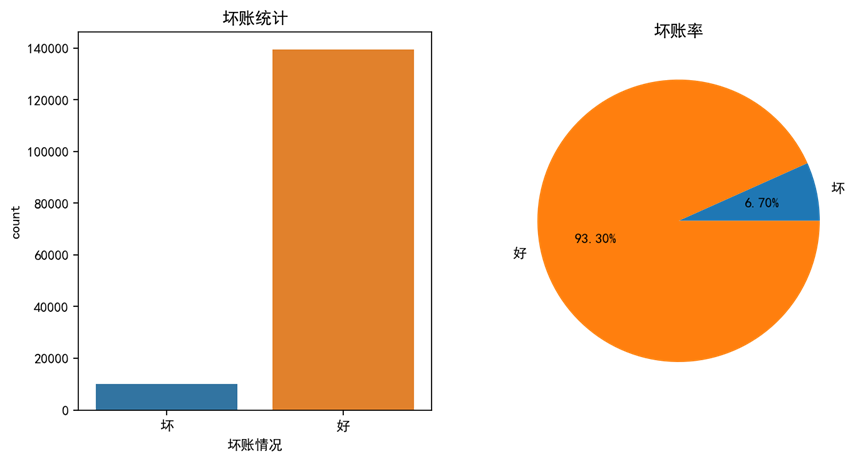
\includegraphics[width=0.6\linewidth]{figures/screenshot002}
	\caption{}
\end{figure}


\subsubsection{解决样本不平衡的方法}
\begin{flushleft}
	\noindent\qquad 我们在采样方法上使用SMOTE算法来平衡样本,以保证之后逻辑回归的准确度。平衡之后的数据如下所示:
\end{flushleft}

\begin{figure}[H]
	\centering
	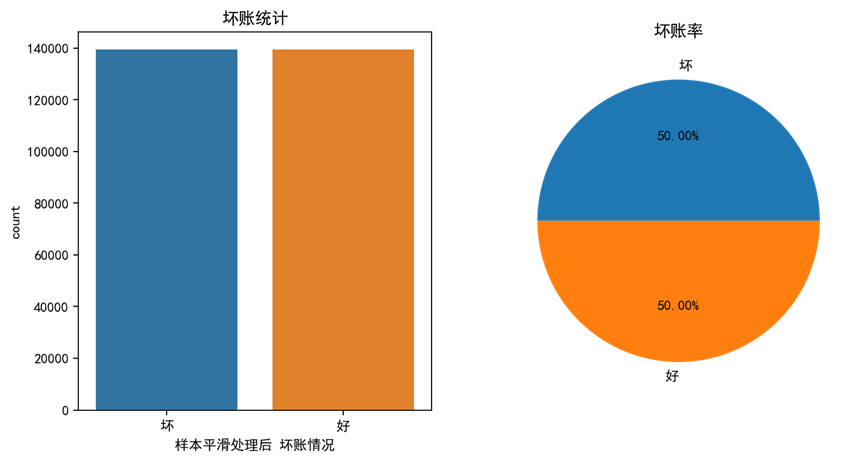
\includegraphics[width=0.6\linewidth]{figures/screenshot003}
	\caption{}
\end{figure}

\newpage
\subsection{分箱}

\subsubsection{为什么分箱}
\begin{flushleft}
	\noindent\qquad 在前面,我们已经对数据进行了重复值处理,缺失值处理,异常值处理,平衡化处理,但是制作评分卡,目的是给各个特征进行分档,以方便业务人员能够根据新客户的信息为其打分,因此需要分箱,其本质是将连续变量转化为离散变量,让组之间的差异尽可能的小,不同组之间的差异尽可能的大,使不同属性之人划分为不同类别,对应不同的分数。\par
	\noindent\qquad 此外,数据特征的分布大多很极端,存在大量的围绕均值波动的数据,同时有少量远离大部分数据存在的极端高值,但是却不能将其归类为异常值,拿月收入MonthIncome来说,存在一部分收入极高,脱离大部分数据分布的值,但是我们却不能判断其为异常,是因为现实中确确实实存在着收入远远高出普通人存在的超高收入人群。\par
	\noindent\qquad 为了避免这些‘异常数据’极端值产生的影响,同时又避免特征中无意义的波动,我们采用分箱的方法,来提高模型的拟合度。
	\noindent\qquad \textbf{关于特征分箱,我们后面会有更详细的解释。}
	
\end{flushleft}
\vspace{2cm}
\begin{figure}[H]
	\centering
	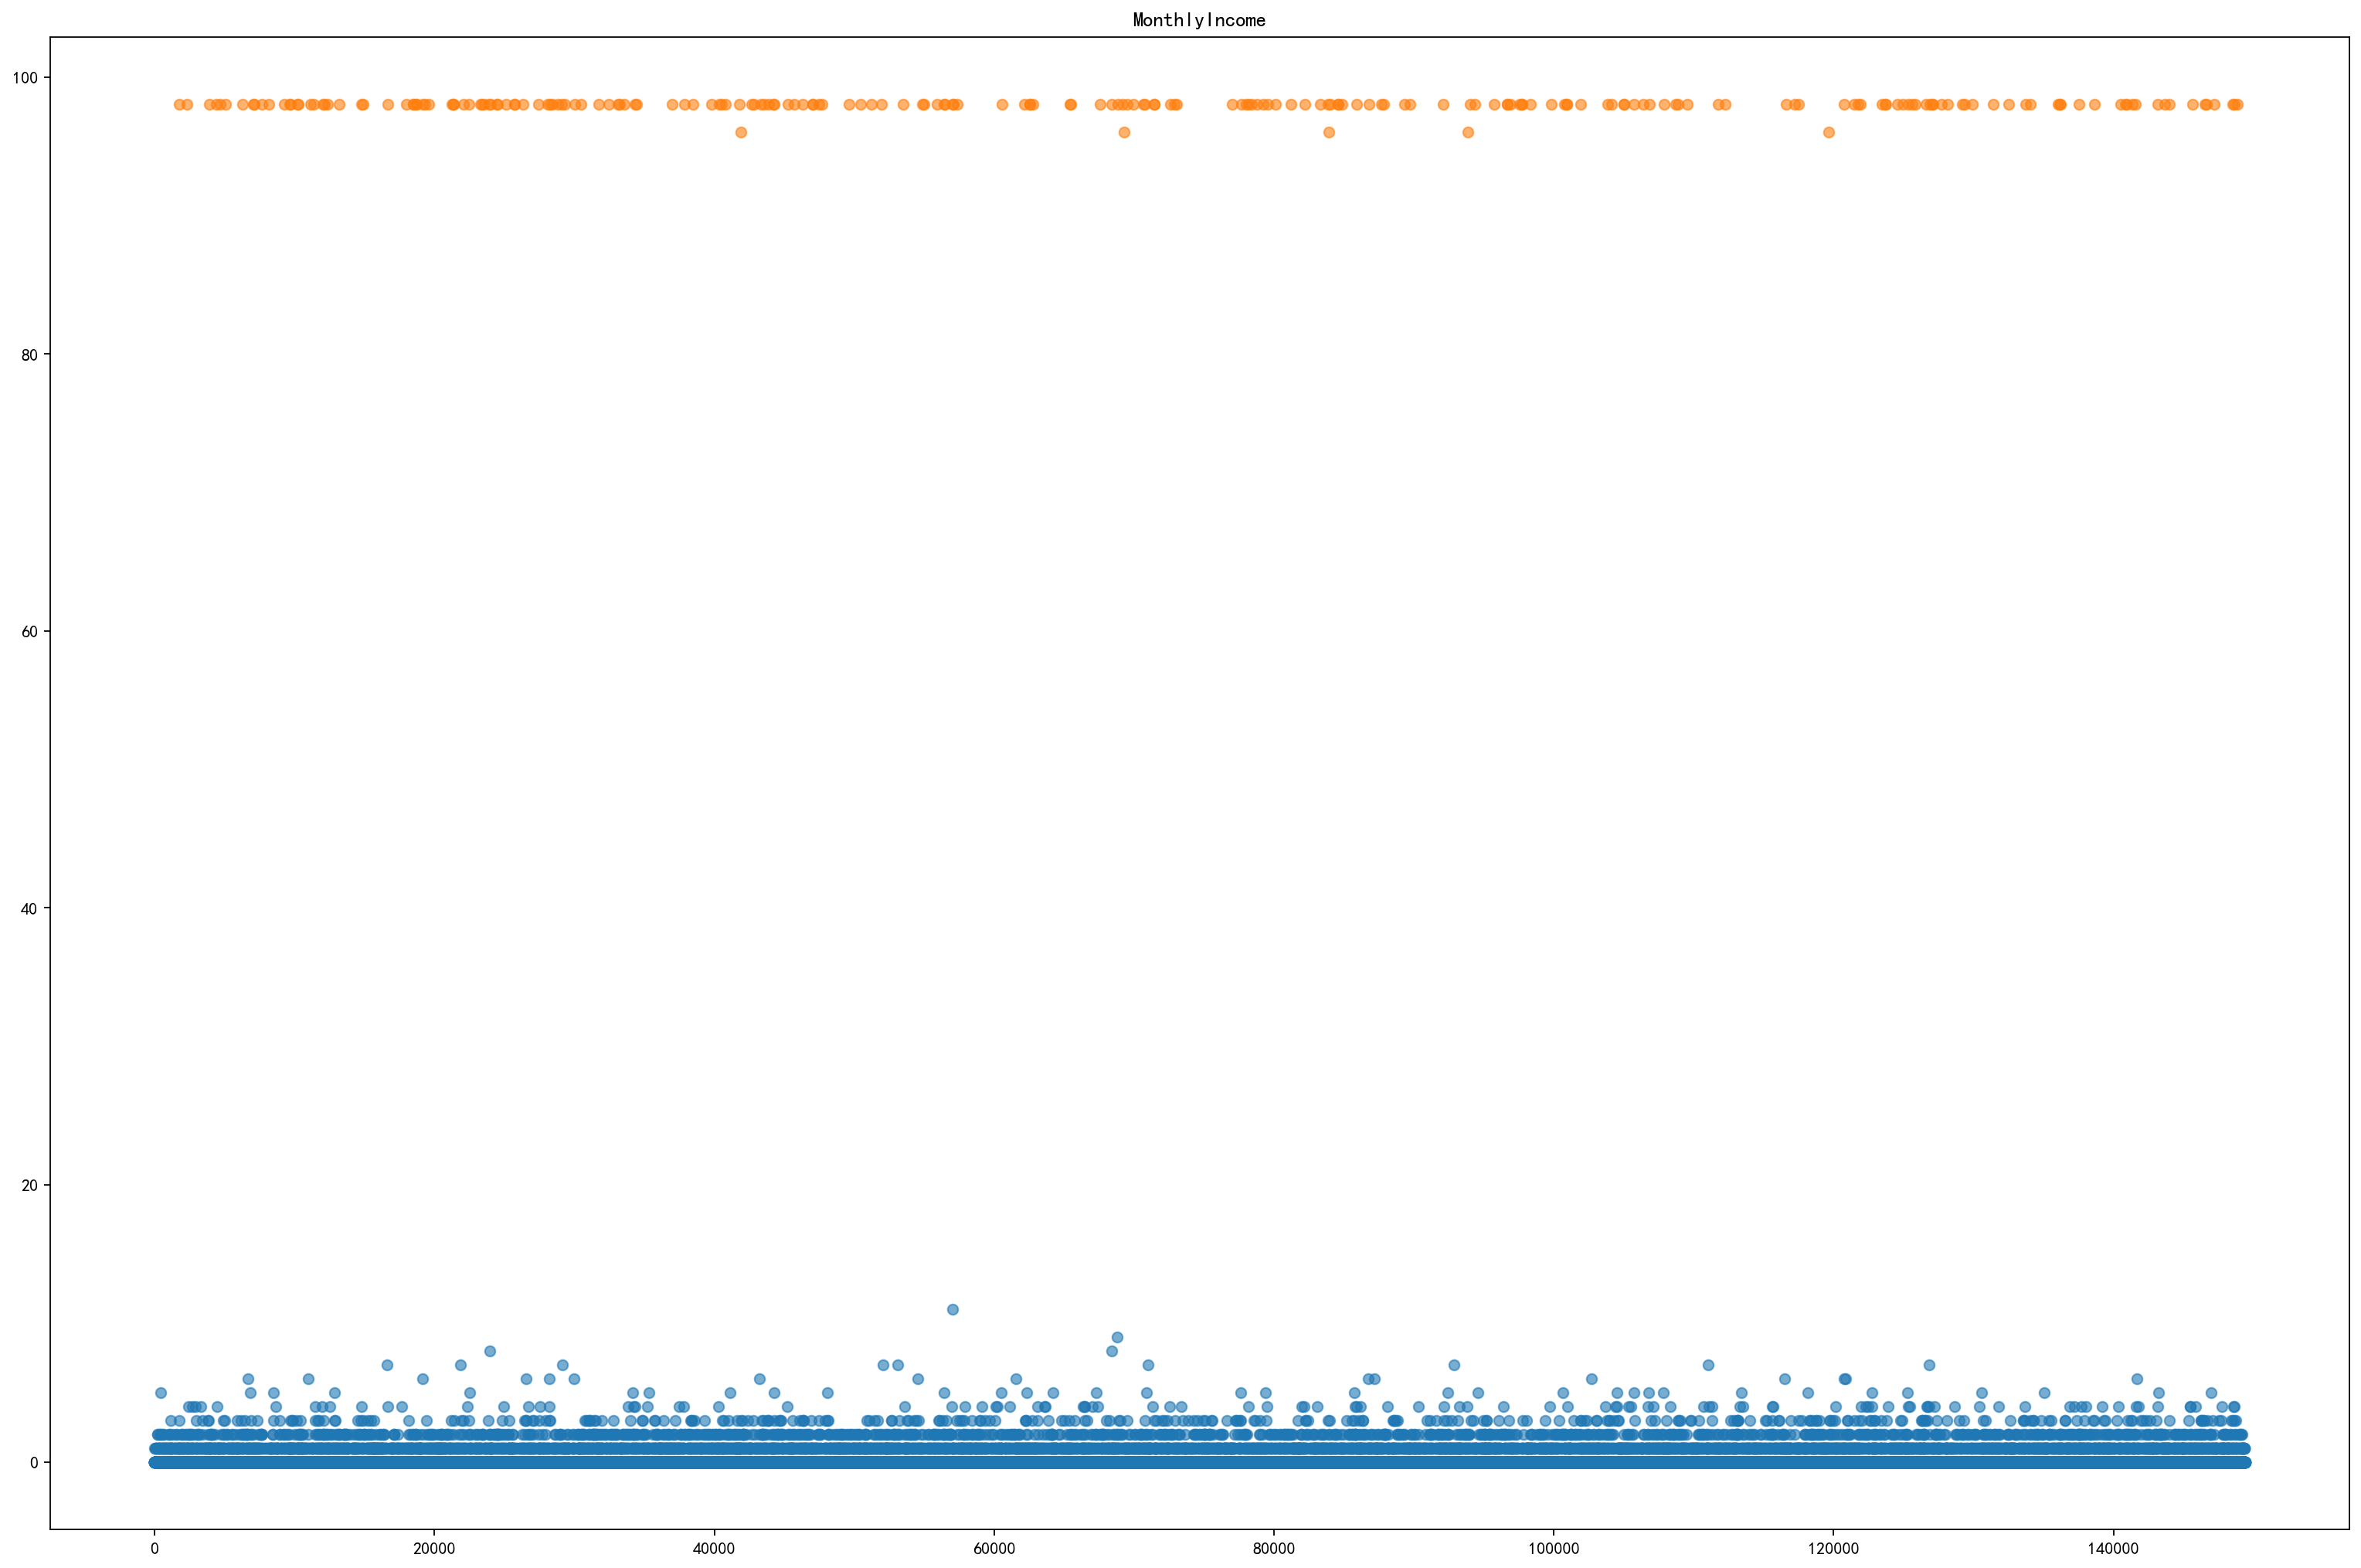
\includegraphics[width=1\linewidth]{figures/MI}
	\caption{}
\end{figure}
\newpage
\subsubsection{关于分箱的个数}
\begin{flushleft}
	\noindent\qquad 改成:首先从业务的角度考虑,分箱数不能过多,其次从模型的角度考虑,分箱数过多会导致IV值变大,对模型的贡献过大,会压缩其他特征影响,这就意味着,数据的微小浮动导致样本属于不同的分段的可能性变大,导致模型不稳定,在这里,我们使用Information value(IV)来进行箱数的确定。\par
	\noindent\qquad \textbf{我们会对特征进行分箱,然后计算每个特征在n个箱子数目下的WOE值,利用IV值的曲线,找出每个特征合适的分箱个数}。\par
	\noindent\qquad Information value(IV):银行业用于衡量特征上的信息量以及特征对预测函数的贡献:
	
\end{flushleft}
\begin{align}
IV=\sum_{i=1}^N (good\%-bad\%)*WOE_i\tag{1}
\end{align}

\begin{flushleft}
	\noindent\qquad N是特征上分箱的个数,i代表每个箱子,good$\%$是这个箱内的非坏账率(标签为0者之比例,银行认为的优质客户),bad$\%$是这个箱子中的坏账率(违约者,标签为1的比例),而WOEi则写作:
\end{flushleft}

\begin{align}\nonumber %排公式
WOE_i=\ln\frac{good\%}{bad\%} \tag{2}
\end{align}

\begin{flushleft}
	\noindent\qquad 银行业中用来衡量违约概率的指标,中文叫做证据权重(weight of Evidence),本质其实就是优质客户比上坏客户的比例的对数。WOE越大,代表了这个箱子里的优质客户越多。而IV是对整个特征来说的,IV的意义如字面(Information value)意思一般,是特征上的信息量以及此特征对模型的贡献,由下表来控制:
\end{flushleft}


\begin{tabular}{|c|c|}
	\hline 
	$IV$ & 特征对预测函数的贡献 \\ 
	\hline 
<0.03	& 特征几乎不带有效信息,对模型没有贡献,这种特征可以删除 \\ 
	\hline 
0.03~0.09	& 有效信息很少,对模型的贡献度低 \\ 
	\hline 
0.1~0.29		& 有效信息一般,对模型的贡献度中等 \\ 
	\hline 
0.3~0.49 	& 有效信息较多,对模型的贡献度较高\\ 
	\hline 
>= 0.5	& 有效信息非常多,对模型的贡献超高并且可疑 \\ 
	\hline 
\end{tabular}  
\begin{center}
	表(4)
\end{center}



\begin{flushleft}
	\noindent\qquad 因此,IV并非越大越好,我们需要找到IV值和箱子个数的平衡点。箱子越少,则IV值必然越小,若存在IV值足够大,并且箱子个数合适的点,那便是理想情况。
\end{flushleft}

\newpage
\subsubsection{卡方分箱}

\begin{flushleft}
	\noindent\qquad 我们希望不同属性的人有不同的分数,因此我们希望在同一个箱子内的人的属性是尽量相似的,而不同箱子的人的属性是尽量不同的,即”组间差异大,组内差异小“。对于评分卡来说,就是说我们希望一个箱子内的人违约概率是类似的,而不同箱子的人的违约概率差距很大,即WOE差距要大,并且每个箱子中坏客户所占的比重(bad$\%$)也要不同。那我们可以使用卡方检验来对比两个箱子之间的相似性,如果两个箱子之间卡方检验的P值很大,则说明他们非常相似,那我们就可以将这两个箱子合并为一个箱子。
	基于这样的思想,我们总结出我们对一个特征进行分箱的步骤:\\
	\vspace{1cm}
	\noindent\qquad·1.我们首先把连续型变量分成一组数量较多的分类型变量,比如,将几万个样本分成100组,或50组\\
	\noindent\qquad·2.确保每一组中都要包含两种类别的样本,否则IV值会无法计算\\
	\noindent\qquad·3.我们对相邻的组进行卡方检验,卡方检验的P值很大的组进行合并,直到数据中的组数小于设定的N箱为止\\
	\noindent\qquad·4.我们让一个特征分别分成[2,3,4.....20]箱,观察每个分箱个数下的IV值如何变,找出最适合的分箱个数\\
	\noindent\qquad·5.分箱完毕后,我们计算每个箱的WOE值,观察分箱效果\\

	\noindent\qquad 这些步骤都完成后,我们可以对各个特征都进行分箱,然后观察每个特征的IV值,以此来挑选特征。
	
	\noindent\qquad 接下来,在构造完算法和定义完WOE和IV函数后(具体算法请看附录),我们以特征"age"和“NumberOfDependents”为例,展示分箱如何完成。\\
	\noindent\qquad 首先,利用卡方分布合并箱体,并画出IV曲线,选择转折点处,使得IV足够大而箱数足够合适,所以这里对于age来说选择箱数为6。而后为其余特征用相同的方法。
	
\end{flushleft}
\begin{figure}[H]
	\centering
	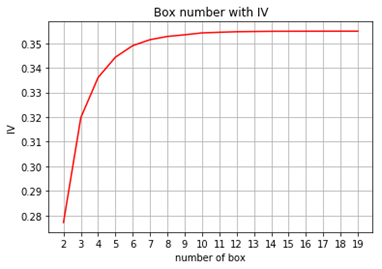
\includegraphics[width=0.7\linewidth]{figures/screenshot004}
	\caption{}
\end{figure}

\newpage

\begin{flushleft}
	\noindent\qquad 前文提到并非所有的特征都能使用卡方分箱,一些类别变量,诸如“家人”就无法分出20组的箱数,这个时候我们只能采用等频分箱的方法,手动得到分箱区间。如特征“”我们通过观察他的分位点分布手动分出的区间为:[0,2,7]。
\end{flushleft}







\begin{figure}[H]
	\centering
	\subfloat[特征分布]{
		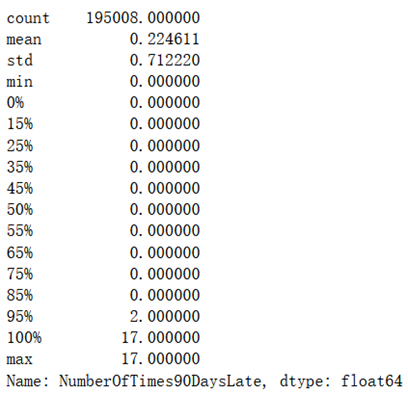
\includegraphics[width=7cm]{figures/screenshot005}
		%\caption{fig1}
	}
	\quad
	\subfloat[类别变量无法使用卡方分箱]{
		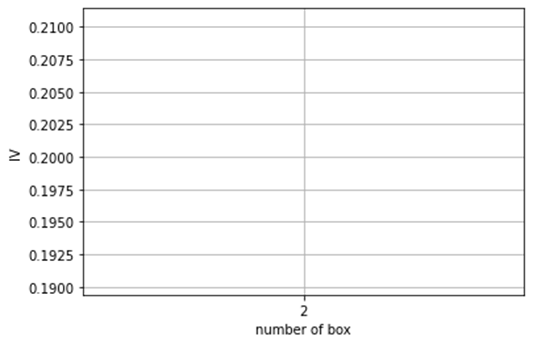
\includegraphics[width=7cm]{figures/screenshot006}
	}

\end{figure}



\subsubsection{WOE编码}
\begin{flushleft}
	\noindent\qquad 前者,我们基于对业务又或对模型的需求进行了分箱,但是模型是没法理解我们分箱之后划分的区间,我们要把他们编码,使得机器可以理解。\\
	\noindent\qquad WOE编码是一种有监督的编码方式,将预测类别的集中度的属性作为编码的数值,所以将特征的值规范到相近的尺度上便是它的优势,但对于我们的模型而言,需要分箱后每箱都同时有好坏样本,我们当然也在算法考虑并实现了这一点
	
\end{flushleft}



\begin{align}
WOE_i = \ln{\frac{good\%}{bad_{rate}\%}}\footnotemark[1] \tag{3}
\end{align}
\footnotetext[1]{good$\%$为不违约人占总体样本的比率。}
\footnotetext[1]{$bad_{rate}\%$ 为违约人数占总体样本的比例。}

\begin{flushleft}
	\noindent\qquad 计算各箱的WOE后,我们以此为依据对数据进行WOE映射,并且覆盖原数据,也就是说,我们接下来将用WOE覆盖后的数据进行建模,这样一来我们便获取到各个箱的分类结果,即评分卡上各个评分项目的分类结果,同样的操作我们也会在测试集上进行。\\
	\noindent\qquad 图2为WOE映射后的训练集 图3为测试集。
	
	
\end{flushleft}

\begin{figure}[H]
	\centering
	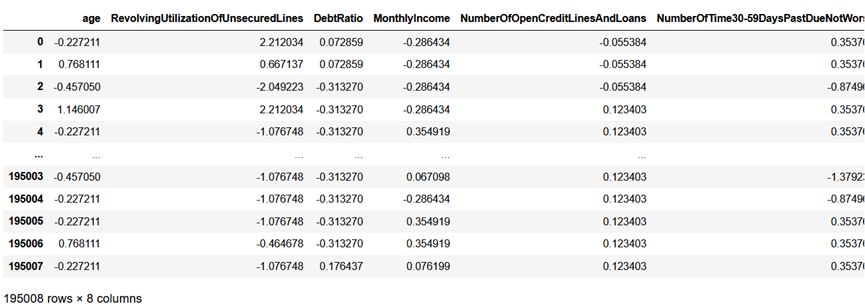
\includegraphics[width=1\linewidth]{figures/screenshot011}
	\caption{训练集:195008行}
	\label{训练集}
\end{figure}
\vspace{3cm}
\begin{figure}[H]
	\centering
	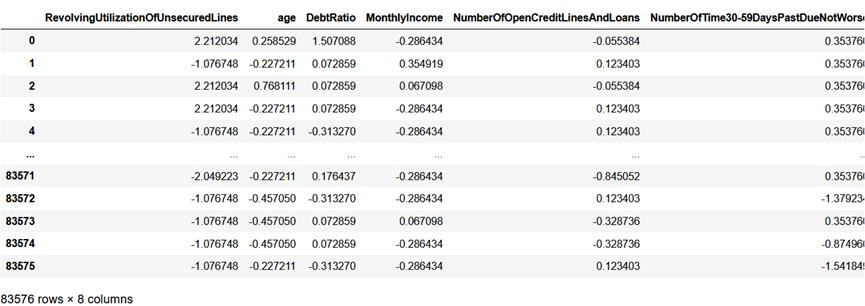
\includegraphics[width=1\linewidth]{figures/screenshot012}
	\caption{测试集:83576行}
	\label{测试集}
\end{figure}



\newpage
\subsection{特征选择}

\subsubsection{单变量分析}
\begin{flushleft}
	\noindent\qquad 依次删除后发现,只有当删除IV值最小的特征(IV=0.04)“”时,MI和DR的IV上升,故决定删去“”,并根据新的IV重新确定分箱,至此,特征变为9列。
	
	
\end{flushleft}
\begin{figure}[H]
	\centering
	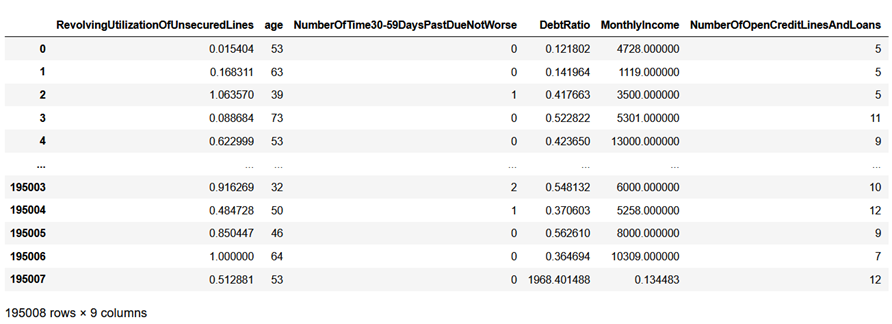
\includegraphics[width=1\linewidth]{figures/screenshot007}
	\caption{}
\end{figure}
\newpage
\subsubsection{皮尔逊检验-热力图}

\begin{flushleft}
	\noindent\qquad 可见特征NumberRealEstateLoansOrLines和NumberOfOpenCreditLinesAndLoans之间的相关系数接近0.5。\\
	\noindent\qquad 对于广义线性模型而言,若特征间存在近似的共线性,会导致拟合参数β估计精度很低,参数估计量经济含义不合理,变量的显著性检验失去意义,可能将重要的解释变量排除在模型之外,模型的预测功能失效。变大的方差容易使区间预测的“区间”变大,使预测失去意义。\\
	\noindent\qquad \textbf{因此删除两者中对模型贡献最小的特征NumberOfOpenCreditLinesAndLoans,模型由9个特征变为8个。}
	
\end{flushleft}
\vspace{1.5cm}
\begin{figure}[H]
	\centering
	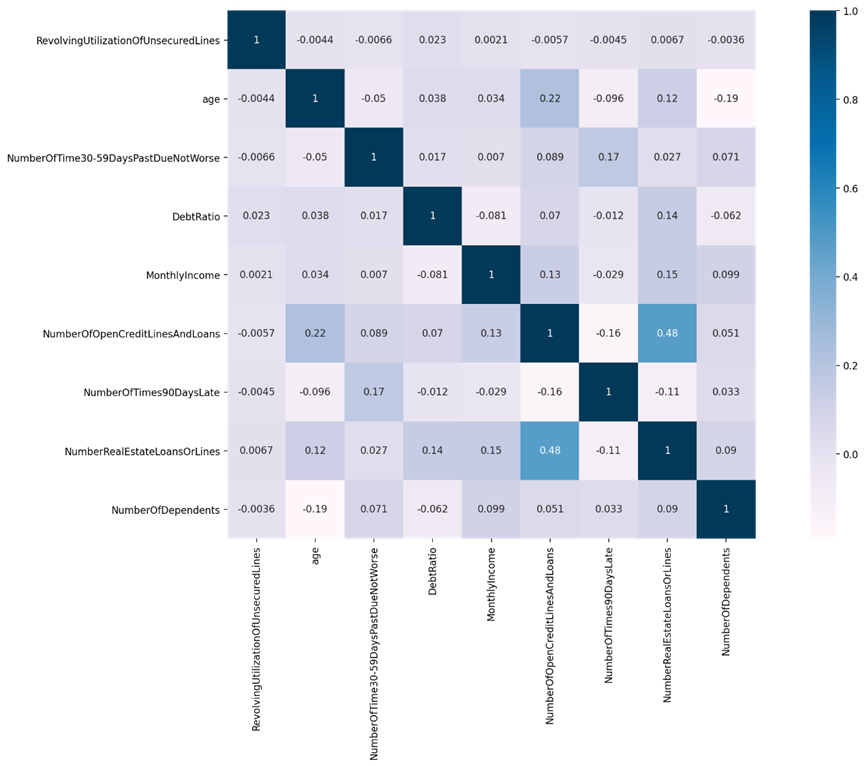
\includegraphics[width=1\linewidth]{figures/screenshot008}
	\caption{热力图}
\end{figure}
\newpage
\subsubsection{多重共线性VIF检验}

\begin{flushleft}
	\noindent\qquad 对数据的8个特征的进行VIF检验,发现其VIF皆小于2.5 ,排除这些特征存在多重共线性的可能
\end{flushleft}

\begin{figure}[H]
	\centering
	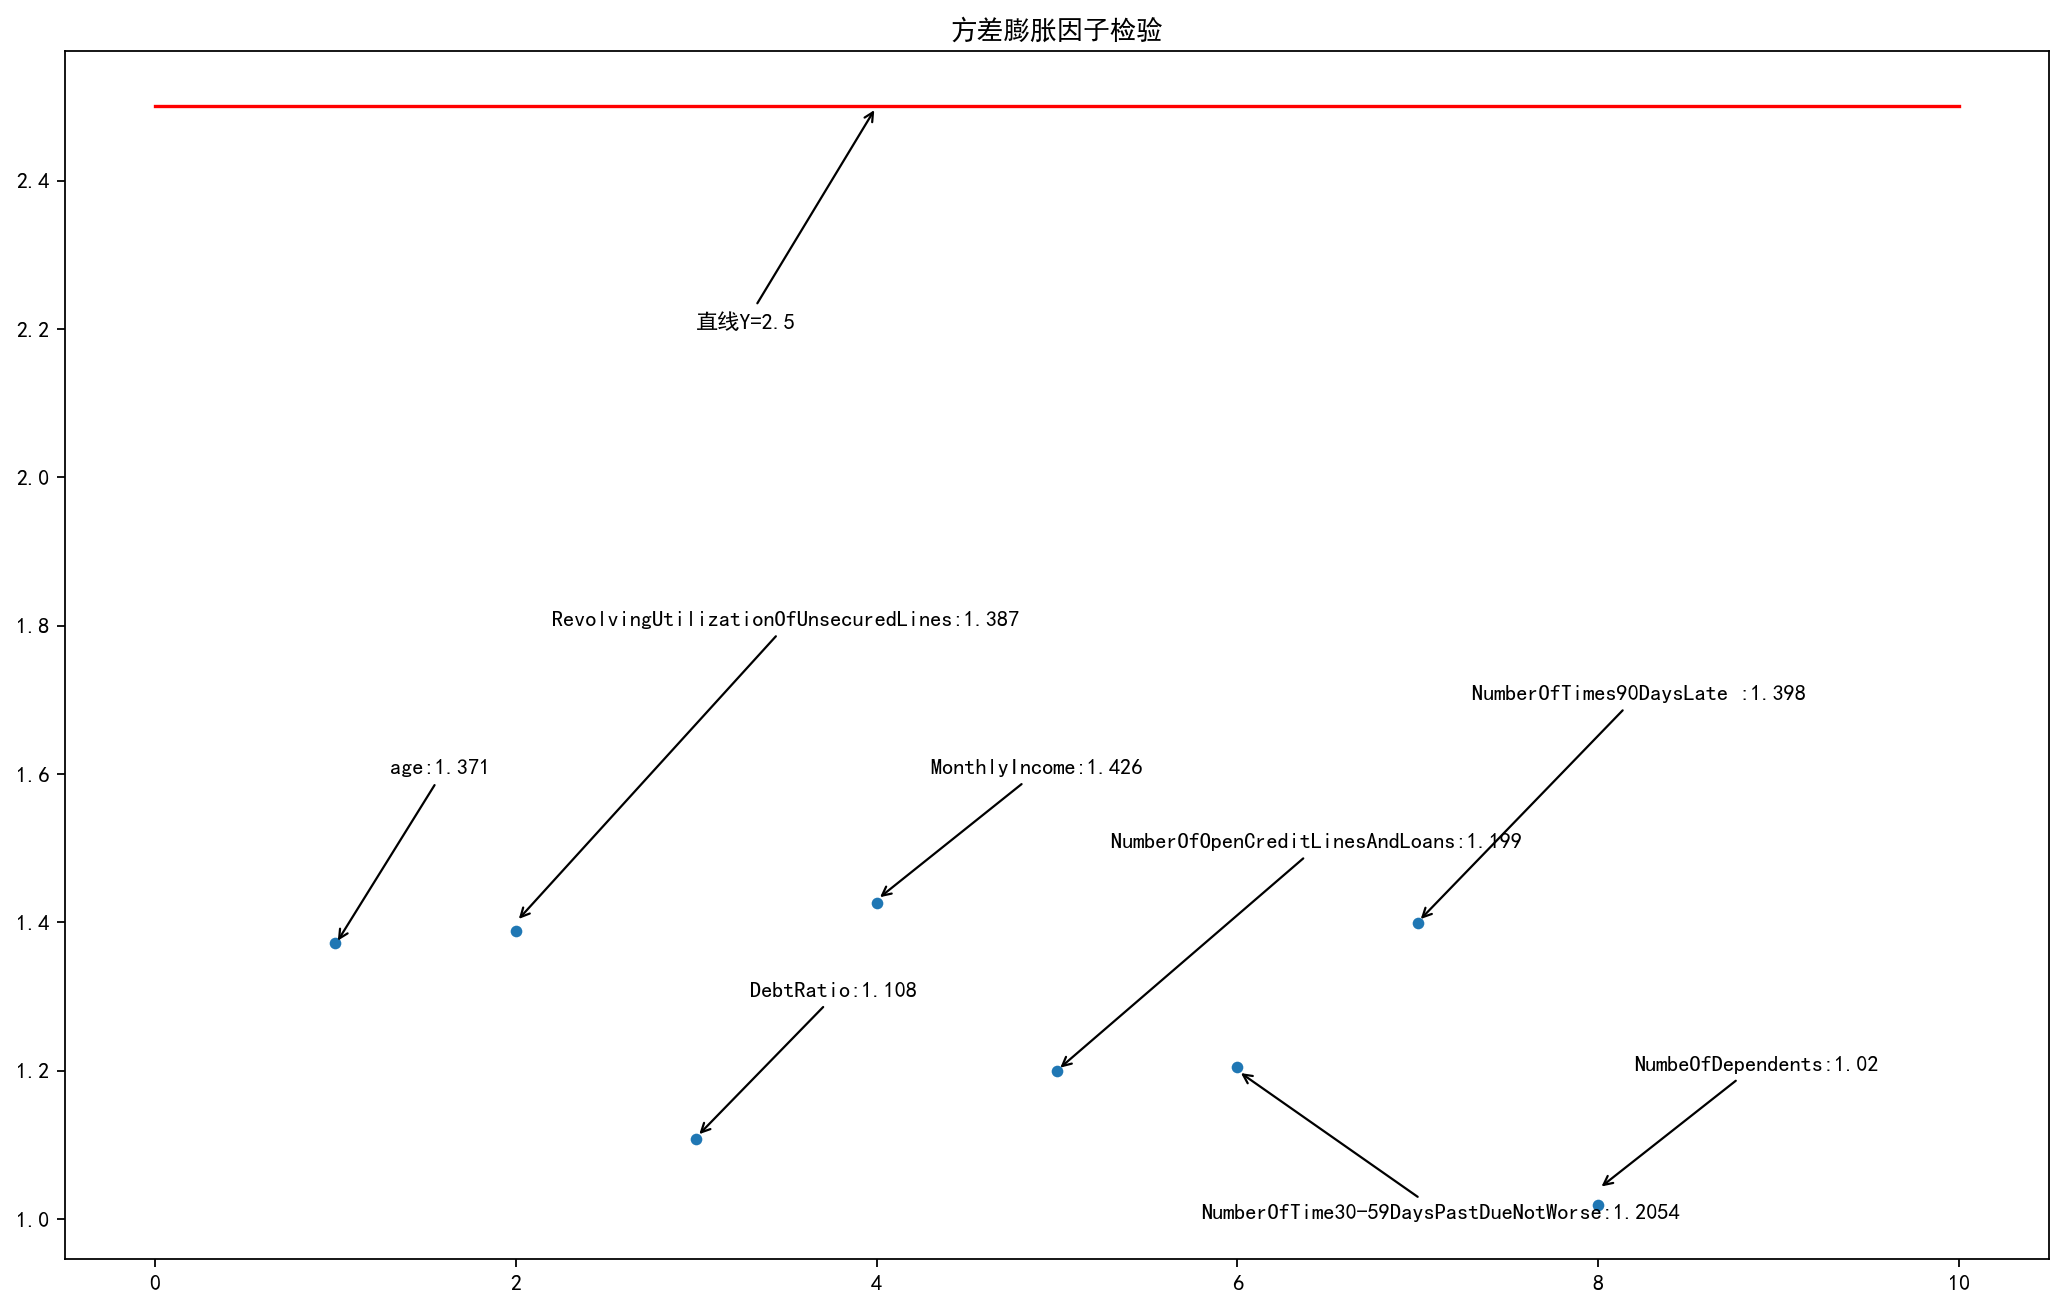
\includegraphics[width=1\linewidth]{figures/index}
	\caption{各特征VIF检验}
\end{figure}


\vspace{1.5cm}

\subsubsection{特征交互性检验}


\begin{flushleft}
	\noindent\qquad 观察交互图,发现产生交互的特征大多为(NumberOfTime60-89DaysPastDueNotWorse与NumberOfTime30-59DaysPastDueNotWorse 与 NumberOfTimes90DaysLate)又或(age与numberofindepende)认为这一类的特征交互对模型没有价值。\\
	\noindent\qquad 亦增加过特征如:‘月收入的平方除以年龄’ 意在分辨出年龄高而收入低者,但模型拟合度不尽人意。(交互图尺寸过于庞大,请于附录中查看)\\
	\noindent\qquad 处理完以后,再次映射各箱的WOE值,最终成为我们建模数据
	
\end{flushleft}
\newpage


\section{模型的建立}

\subsection{信用卡与评分卡建立}
\subsubsection{信用分模型}


\begin{flushleft}
	\noindent\qquad 目前有$n$个样本,每个样本表示一个贷款客户的信息。则第$i$个样本表示为$\{x_i.y_i\}$,其中 $y\in \{0,1\}$ 0代表正常,1代表逾期
	写成矩阵的形式:
	
	
\end{flushleft}

$$X = \left \{ 
\begin{aligned}
1  &&  x_{1,1} && x_{1,2} && ... && x_{1,r} \\
1  &&  x_{2,1} && x_{2,2} && ... && x_{2,r} \\ 
...  &&  ... && ... && ... && ... \\  
1 &&  x_{n,2} && x_{n,3} && ... && x_{n,r} \\
\end{aligned}\right\}  
$$
$$
Y = (y_1,y_2,...,y_n)^T 
$$




\begin{flushleft}
	\noindent\qquad 对客户$i$而言,如果其逾期的概率是$p_i$,那么其正常的概率就是$1-p_i$ ,一个客户要么逾期要么正常,逾期和正常的概率之和必然是1。
	因为需要根据$X$评估用户$i$是否会逾期。所以可以考虑使用最常见的广义可加模型,其中线性模型最为简单。
	如下所示::
	
\end{flushleft}



\begin{align}
	z_i=\beta_0+\beta_1 x_{i,1}+\beta_2 x_{i,2}+...+\beta_r x_{i,r} \tag{4}
\end{align}



\begin{flushleft}
	\noindent\qquad 另外,又考虑到概率$p_i$的值域是$[0,1]$区间,希望输出的函数值在这个值域。因此再嵌套一层函数以变换值域: 
	
\end{flushleft}



\begin{align}
    P_i=\frac{e^{z_i}}{1+e^{z_i}}=\frac{1}{1+e^{-z_i}}  \tag{5}
\end{align}


\begin{flushleft}
	\noindent\qquad 显然,上式的值域一定是在[0,1]区间的,这里使用logsitic函数是因为$e^{z_i}$在微分求导上更便利。
	样本$x_i$对应的借款人,可能是逾期,也可能是正常,可以用一个公式同时表示这两种情况:\\
	
	\begin{align}  %自动编号
		 &P_i=P(y_i|x_i\beta_i) = (p_i)^{y_i}(1-p_i)^{(1-y_i)}  \notag\\  \tag{6}
		 &y_i \in \{0,1\} 
	\end{align}
	 
	\noindent\qquad 对n个样本而言,样本之间是相互独立的,因此对所有样本而言,其全体概率是:$L(\beta)=\prod_{i=0}^nP_i$
	\noindent\qquad 那么我们就需要对其中的参数$\beta_j$进行估计,也就是让$L(\beta)$的值最大,这里采用的是极大似然估计,这样就可以得到损失函数:\\
	
	\begin{align}  %自动编号
	min·ln^{L(\beta)} =-\frac{1}{m}\sum(y_i\frac{1}{p_i}+(1-y_i)\frac{1}{(1-p_i)})  \tag{7}
	\end{align}
	
	

	\noindent\qquad 得到损失函数以后,我们再使用梯度下降法求得近似最优解。
	
\end{flushleft}

\subsubsection{评分卡模型建立}

\begin{flushleft}
	\noindent\qquad 评分卡的分值分配,由比率决定。例如,一个评分卡可以设定,评分每降低$20$分,违约的比率升高一倍,$600$分账户的违约比率是$620$ 分账户的两倍。每个得分对应一个特定的违约比率,便于控制预期违约账户。
	
\end{flushleft}

\begin{align}  %自动编号
Odds=\frac{p_i}{1-p_i} \tag{8}
\end{align}

\begin{flushleft}
	\noindent\qquad $Odds$(几率):不违约概率与违约概率的比值
	公式$odds$做个变形,也就有:
	
\end{flushleft}


\begin{align}  %自动编号
p_i=\frac{Odds}{1+Odds}  \tag{9}
\end{align}



\begin{flushleft}
	\noindent\qquad 评分卡的信用分计算:
	
\end{flushleft}



\begin{align}  %自动编号
Score=A-B\ln(Odds)  \tag{10}
\end{align}


\begin{flushleft}
	\noindent\qquad 其中,A和B是常数。如果违约率$p$很小,那么Odds是一个正的小数,比如0.01、0.02,表示逾期概率很低,此时$ln(Odds)$是大的负数,$Score$的分数高。反之可知$Score$的分数低。\\
	\noindent\qquad 我们使用PDO(指定的违约概率翻倍的分数)方法来计算A和B:
	
	\vspace{1cm}
	\noindent\qquad·1.设定某个比率为$\theta_0$的对应的分值是$p_0$,然后,比率为$2\theta_0$的点的分值是$p_0+PDO$。\\
	\noindent\qquad·2.将上述两个设定带入公式,有如下两个等式\\
	

	
	
\end{flushleft}


\begin{align}  %自动编号
p_0=A-B\ln(\theta)  \notag \\  \tag{11}
p_0+PDO=A-B\ln(2 \theta)  
\end{align}


	\vspace{1cm}
\begin{flushleft}
	\noindent\qquad 两个等式联合求解,可得:
	
\end{flushleft}


\begin{align}  %自动编号
B&=\frac{PDO}{\ln(2)} \notag \\  \tag{12}
A&=p_0+B\ln(\theta_0)   
\end{align}

\begin{flushleft}
	\noindent\qquad 计算示例,违约比$Odds=\frac{1}{60}$的时候,是合理的违约比,此时对应的分值是$p_0=600$分,违约比每翻倍,分数变小$20$分,也就是PDO=$20$。那么,根据上述公式可以求出$A=481.86$,$B=28.85$,也就是$Score=481.89-28.85ln(Odds)$。如果$Odds=\frac{1}{30}$,增加一倍,则$Score$经过计算可得是$580.01$,四舍五入后是$580$,\\
	\noindent\qquad 信用分分值的分布,由A、B和“理论”的Odds三者决定。“实际”的Odds的分布由$\beta_j(j=0,1,...r)$决定。因此,对$\beta_j$的计算,跟A 和B的计算无关。
	
\end{flushleft}



\newpage
\subsection{分类模型的选择}
\begin{flushleft}
	\noindent\qquad 对于分类问题,在机器学习领域中已经有许多成熟的算法可以用来解决。但是对于一个未知的样本集,是没有办法提前确定一套最好的方案的,目前采用最广泛的方案是使用交叉验证集法来进行模型的选择。\\
	\noindent\qquad 在这里,我们横向比较了目前比较流行的三种分类模型的分类能力,这三个模型分别为Knn(K-NearestNeighbor ,最近邻算法)、SVM(Support Vector Machine,支持向量机),LR(logstic Regression,逻辑斯蒂回归),受限于机器的性能,我们只选取了2$\%$的样本(即2000条数据)进行检测。
\end{flushleft}
\subsubsection{KNN模型}
\begin{flushleft}
	\noindent\qquad 在此数据集中,我们检测了三个KNN模型的准确度,从中挑选了准确度最高的一种,加入到交叉验证模型组中,这三组分别为:\\
	\vspace{1cm}
	\textbf{
	\noindent\qquad-普通KNN\\
	\noindent\qquad\noindent\qquad 近邻样本数:10\\
	\noindent\qquad\noindent\qquad 准确率:0.7049999999999998\\
	\noindent\qquad-带权重的KNN\\
	\noindent\qquad\noindent\qquad 近邻样本数:10,权重模式:“distance”\\
	\noindent\qquad\noindent\qquad 准确率:0.721\\
	\noindent\qquad-指定半径的KNN\\
	\noindent\qquad\noindent\qquad 近邻样本数:10,半径为500\\
	\noindent\qquad\noindent\qquad 准确率:0.48999999999999994\\
}
\end{flushleft}

\
\subsubsection{SVM模型}

\begin{flushleft}
	\noindent\qquad 在这里,我们使用了高斯核函数,并且使用GridSearch参数最优化确定参数gamma:
	\textbf{准确度:0.7785}
	
\end{flushleft}
	\vspace{1cm}
\subsubsection{Logsitic模型}
\begin{flushleft}
	\noindent\qquad 在这里我们使用L2正则化的逻辑斯蒂模型:\\
	\textbf{准确率:0.78}
	
\end{flushleft}

\newpage

\subsection{三种模型的学习曲线比较}

\subsubsection{Logsitic回归}
\begin{figure}[H]
	\centering
	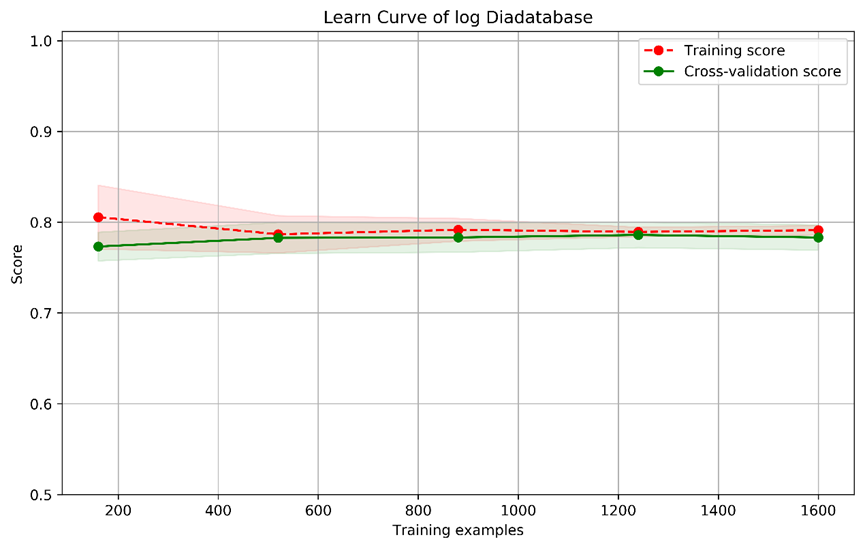
\includegraphics[width=0.7\linewidth]{figures/screenshot013}
	\caption{}
\end{figure}

\subsubsection{SVM}
\begin{figure}[H]
	\centering
	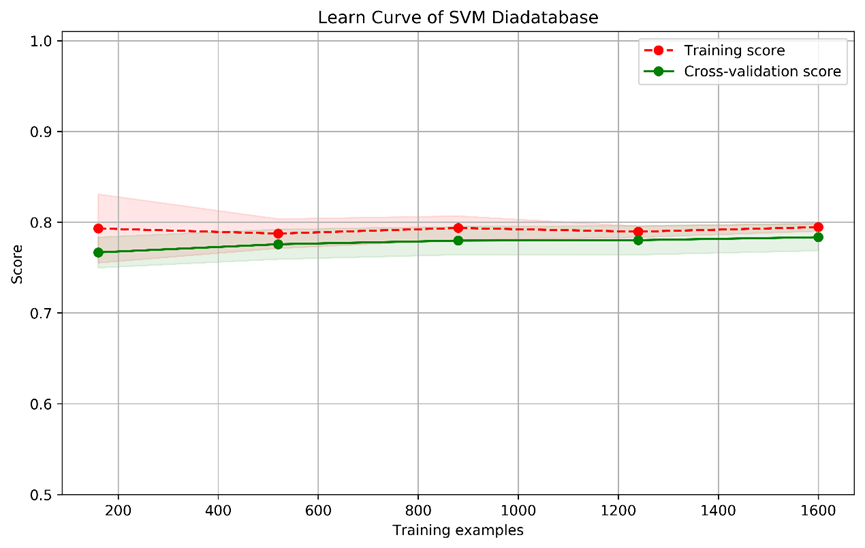
\includegraphics[width=0.7\linewidth]{figures/screenshot014}
	\caption{}
\end{figure}

\subsubsection{带权重KNN}
\begin{figure}[H]
	\centering
	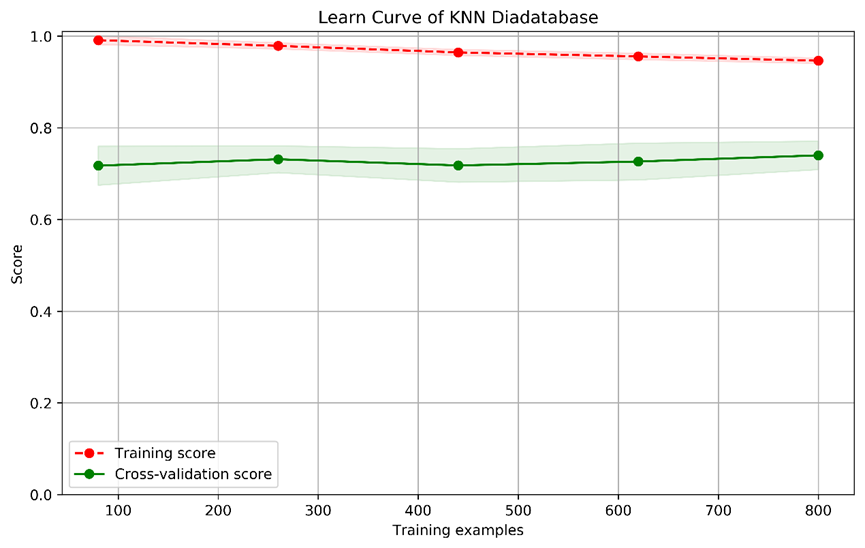
\includegraphics[width=0.7\linewidth]{figures/screenshot015}
	\caption{}
\end{figure}


\newpage
\subsection{Logsitic模型}






\subsubsection{参数调整}
\begin{flushleft}
	\noindent\qquad 对于逻辑斯蒂回归模型,主要有两个参数可以优化,一个是正则化参数C,另一个是迭代轮数,前者属于超参数调整,因为不同的正则化参数,对于损失函数的惩罚力度是不同的,而由于在这里的逻辑斯蒂回归使用的是梯度下降法寻找损失函数最小值的策略,所以容易陷入局部最优,所以,多次迭代选择不同的初始点可以一定程度改善这个问题\\
	\noindent\qquad 对于正则化参数C,使用线性搜索法,从0.0到0.3,步长为0.003,逐一搜索:
	
\end{flushleft}
\begin{figure}[H]
	\centering
	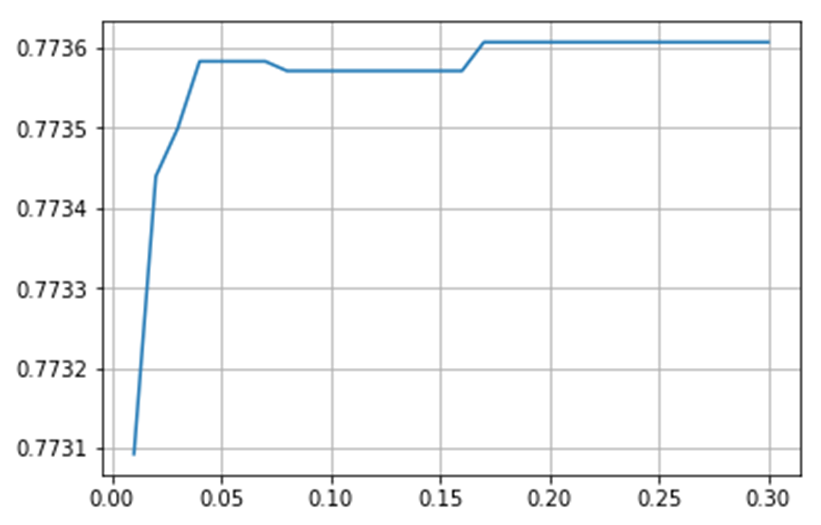
\includegraphics[width=0.7\linewidth]{figures/screenshot016}
	\caption{}
\end{figure}

\begin{flushleft}
	\noindent\qquad  对于迭代轮数:我们一共选择了6轮来观察最优的那个轮数
\end{flushleft}

\begin{figure}[H]
	\centering
	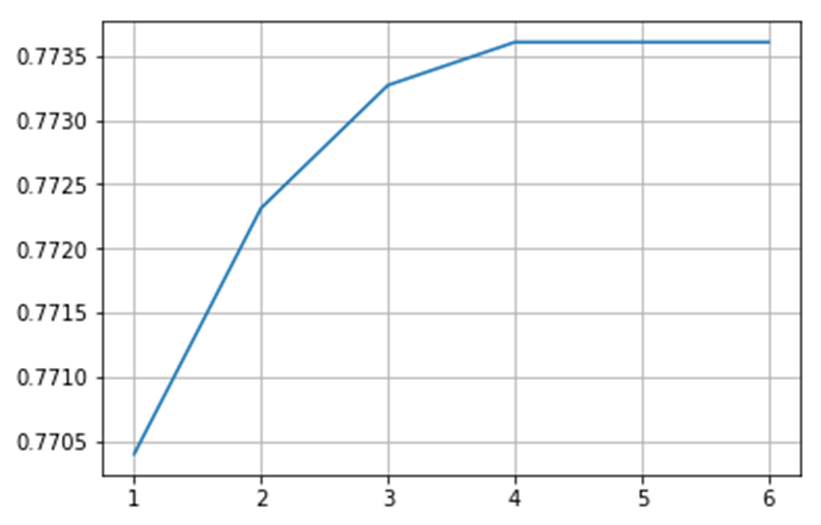
\includegraphics[width=0.7\linewidth]{figures/screenshot018}
	\caption{}
\end{figure}

\begin{flushleft}
	\noindent\qquad  从上面两张图片中以看出,模型的性能到达瓶颈,无论是调整正则化参数还是增加轮数,模型的准确度均会收敛于0.7736左右,不过这为我们下一步的优化指明了方向(L2正则化(lasso)倾向于删掉变量,而随着C的增大,模型的准确度上升说明,更少的特征系数被压缩到0,或者说越少的特征被删除,可能会导致模型的准确率上升,所以需要增加特征来提高准确度。)
	
\end{flushleft}

\subsubsection{性能评估}

\begin{flushleft}
	\noindent\qquad 对于一个分类器,光用准确率进行评判其实是不准确的,比如说,有99个人不违约,但是有一个人违约,这时分类器判断100个人全部不违约,那么这个模型的准确率就是99$\%$.但是这样的分类器是没有意义的,这个时候我们需要使用ROC曲线来评判模型
\end{flushleft}

\begin{figure}[H]
	\centering
	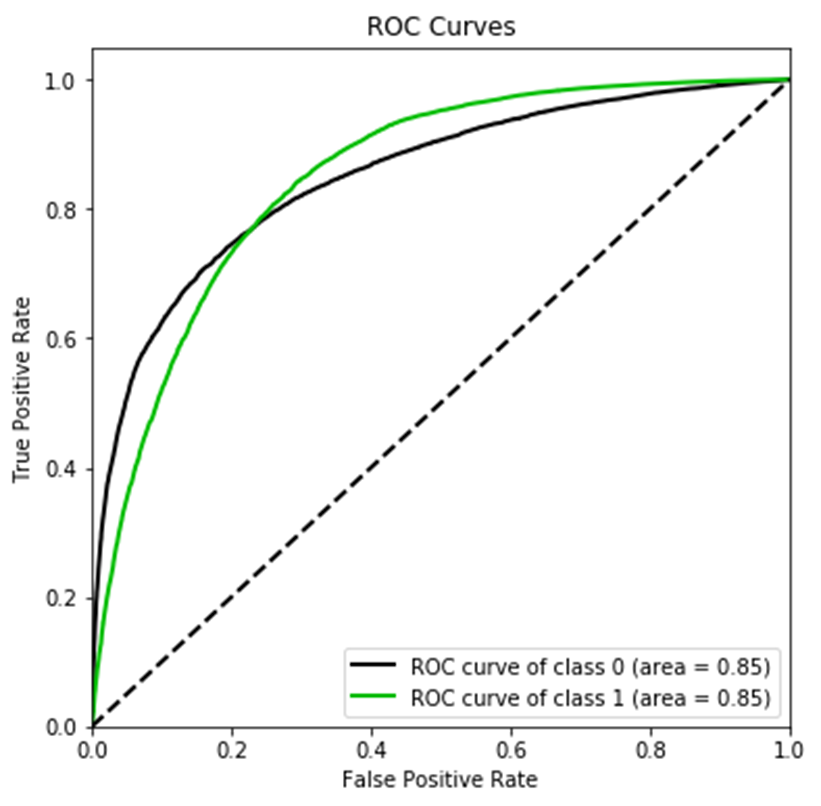
\includegraphics[width=0.7\linewidth]{figures/screenshot019}
	\caption{}
\end{figure}

\begin{flushleft}
	\noindent\qquad 简而言之,ROC曲线下面积即AUC越大,证明模型的泛化能力越好,越有用,在这里,判断为“不违约”的AUC与“违约”的AUC是相等的为0.85,说明模型的分类能力较强,当然,一般地我们希望分类器得到的分类结果是完全正确的,也就是正例样本全部都能够被检测出来,也就是全部都是真正例,或者真反例,这个时候TPR=1且FPR=0,反应在图像上好的分类器的折线应该更加接近左上角。从我们的图像上可以看出,当把把阈值设为0.5时,可以看出模型更擅长分类正例(即“违约”)。
\end{flushleft}
\newpage
\section{分析结果}
\begin{flushleft}
	\noindent\qquad 根据信用评分卡模型建立部分,我的得到了信用评分表,如下所示:
	其中要注意的是,分值越低代表信用越高
\end{flushleft}


\begin{figure}[H]
	\centering
	\subfloat[评分表第一部分]{
		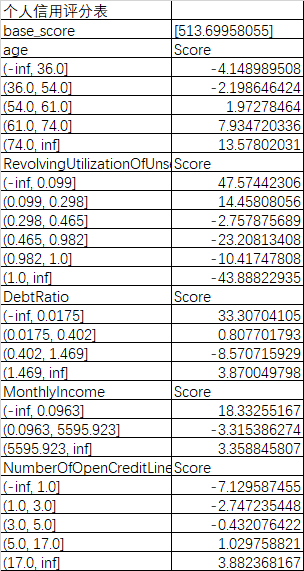
\includegraphics[width=7cm]{figures/pin1}
		%\caption{fig1}
	}
	\quad
	\subfloat[评分表第二部分]{
		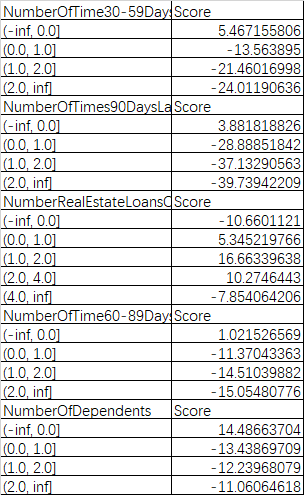
\includegraphics[width=7cm]{figures/pin2}
	}
	
\end{figure}
\begin{center}
	表(5)
\end{center}

\newpage
\subsection{评分卡的解释}

\begin{flushleft}
	\noindent\qquad 以age为例, 新客户的age信息在0-36的区间,则有-4.148的分数,在36到54岁的区间上,则有-2.198的分数,在54到61岁则有1.972的分数,以此类推,将每一个特征进行配对,得分,合计分数越高则说明其信用程度越高,越不容易违约。
	\noindent\qquad	可以看到age特征中,年龄越高,得分越高,越不容易违约,而在数据中(见可视化图25)也与预想的分布相同.
\end{flushleft}
\vspace{2cm}
\begin{figure}[H]
	\centering
	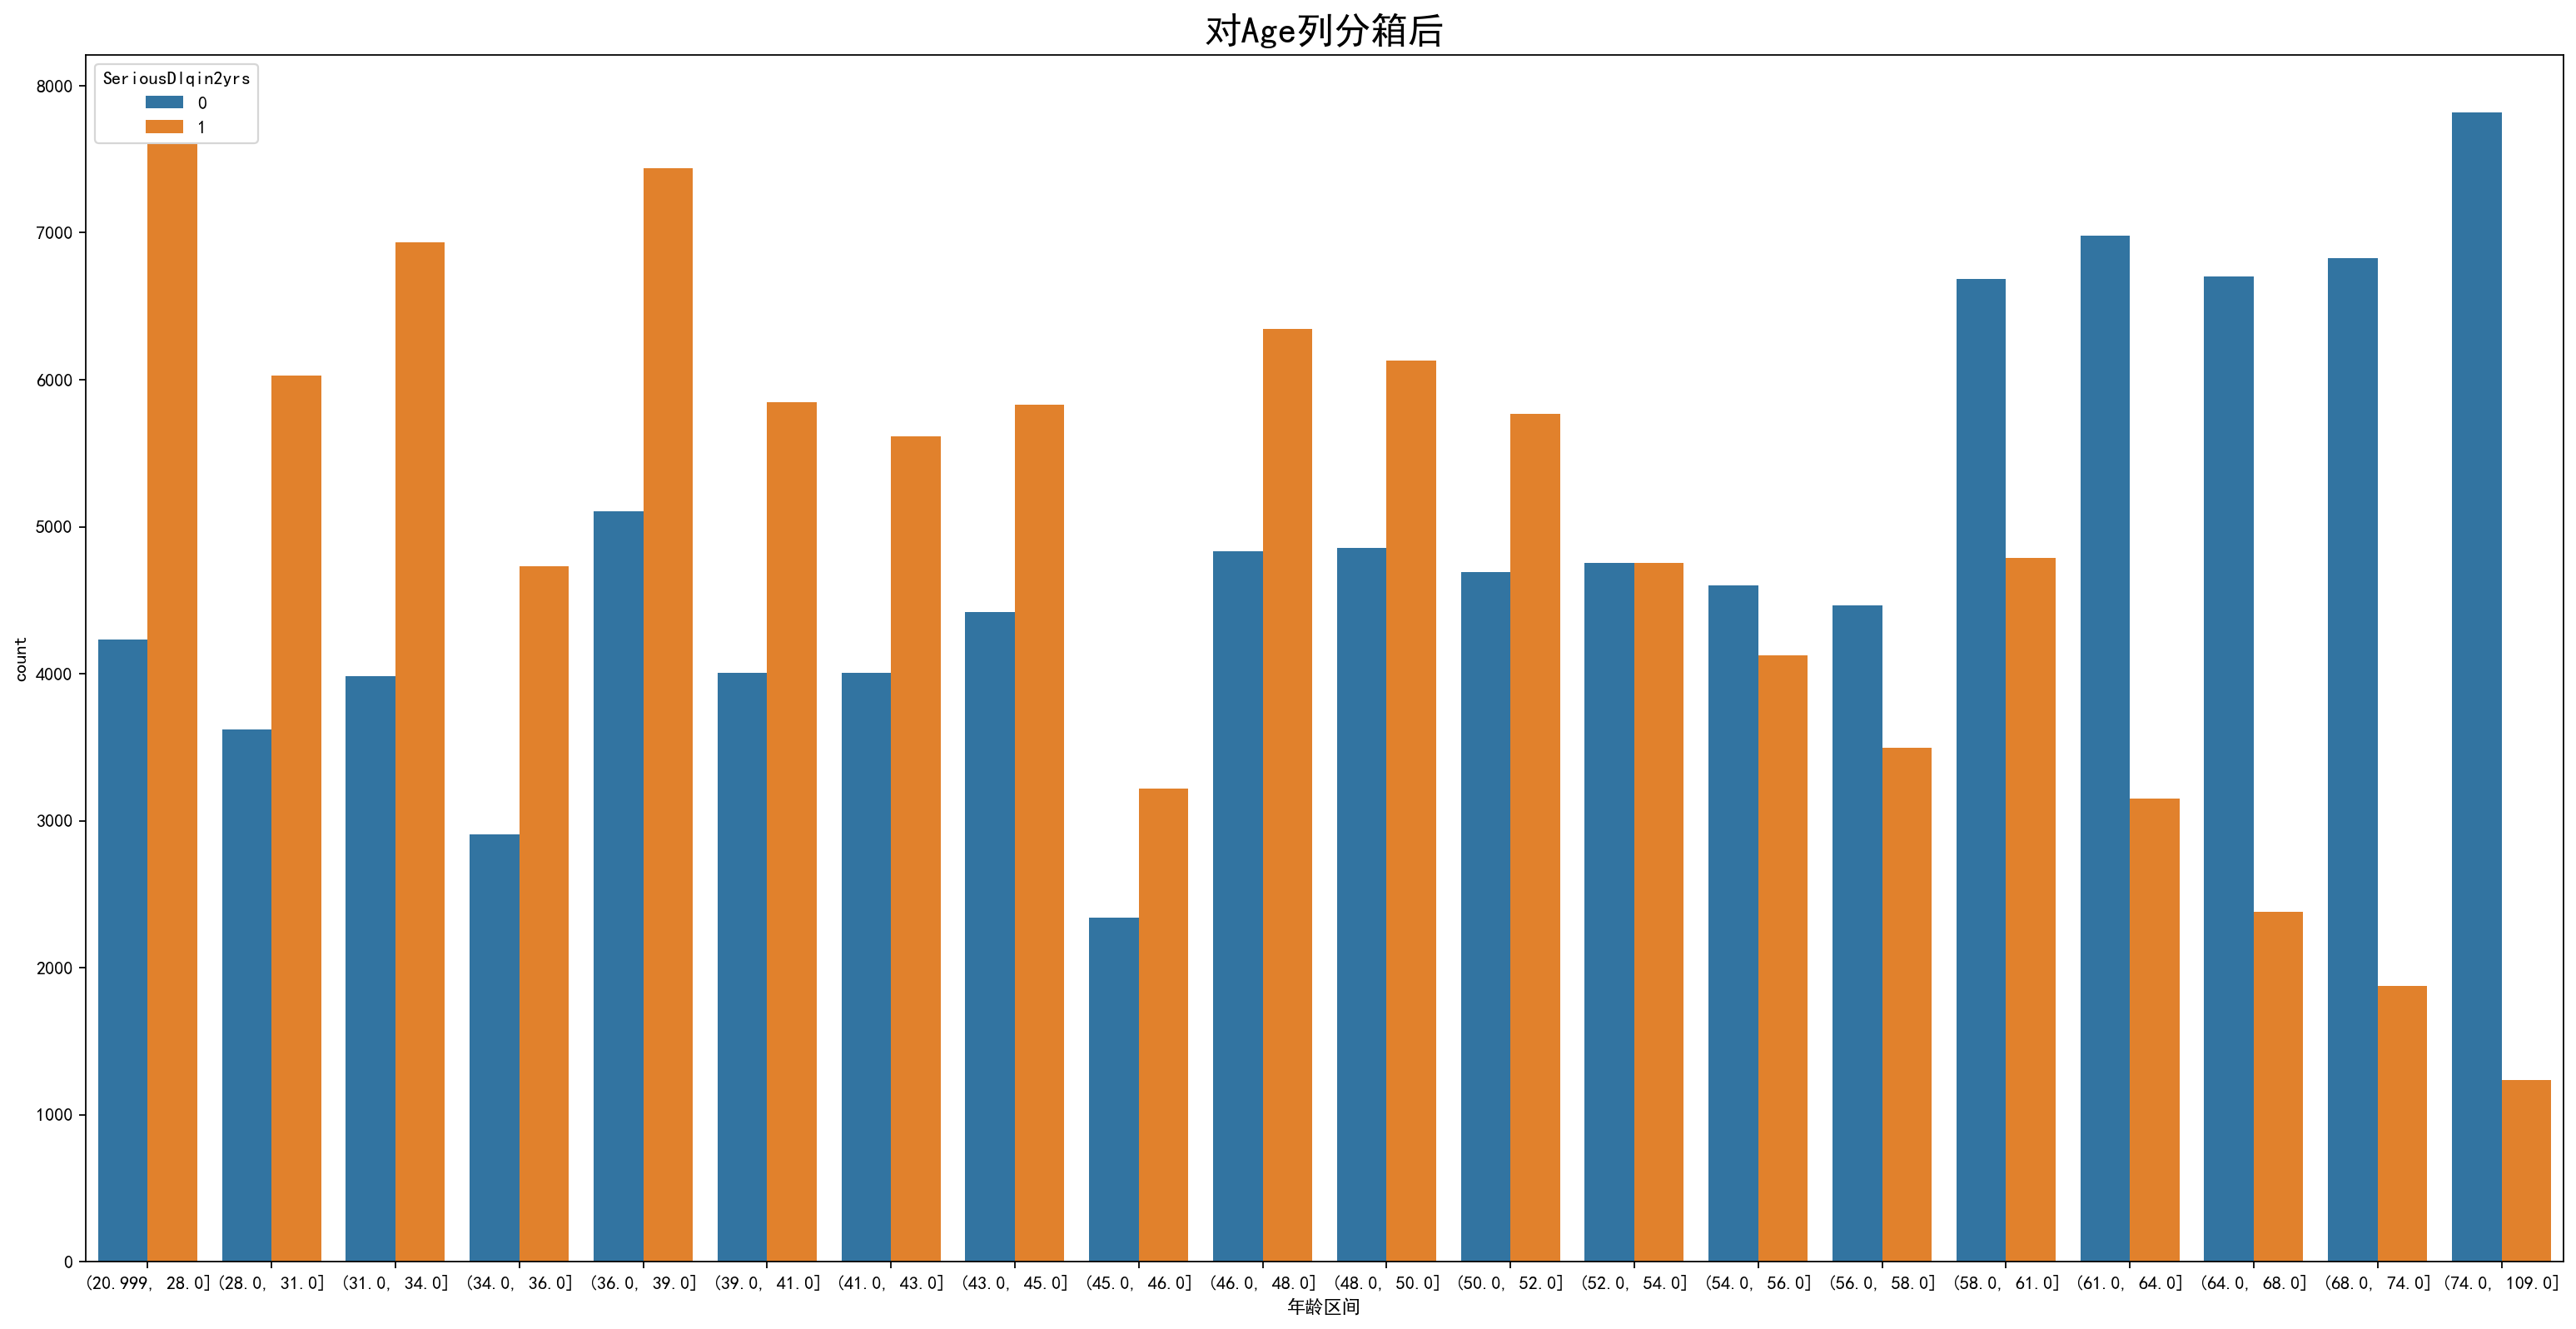
\includegraphics[width=1\linewidth]{figures/age}
	\caption{}
	\label{年龄越大,违约人数占比越小}
\end{figure}
\vspace{2cm}
\begin{flushleft}
	\noindent\qquad 因此,说明我们的评分卡是有者不错的解释性的。
\end{flushleft}






\newpage
\subsection{抽取样本用评分卡制作分数}

\begin{flushleft}
	\noindent\qquad 我们抽取了三个样本,得到他们的分数如下:
	
	
\end{flushleft}
\begin{figure}[H]
	\centering
	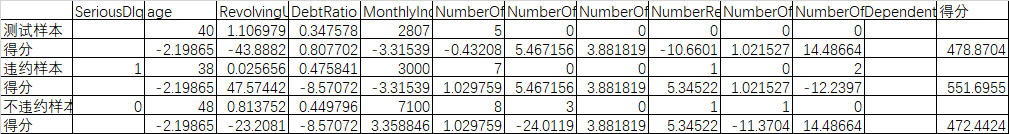
\includegraphics[width=1\linewidth]{figures/pin3}
\end{figure}
\begin{center}
	表(6)
\end{center}

\begin{flushleft}
	\noindent\qquad 从中可以明显的看到,不违约样本的得分高于违约样本,其中测试样本为,隐性不违约样本(隐性即隐藏其是否违约的标签),求出得分后,发现与不违约样本分数相近,经检查,的确为不违约样本,故我们的评分卡效果良好,可以作为银行业务员判断客户违约概率的辅助手段,
	
\end{flushleft}








\section{优点与创新}

\begin{flushleft}
	
\noindent\qquad  创新点:\\
1.横向比较了不同分类模型的优点,具有一定的指导意义。\\
\noindent\qquad  优点:\\
1.使用分箱法,提高了模型的稳定性,避免特征中无意义的波动,提高了模型的鲁棒性:避免了极端值的影响\\

2.使用卡方分箱,一般的信用卡评分建模,使用的分箱方法是等频分箱,等频分箱没有受到目标变量的影响,主观性太强,而使用卡方分箱,则是考虑到,特征对于目标变量的“价值程度”,遵循统计学中“组内差异小,组间差异大”的原则。\\

3.模型的泛化能力强,具有推广的价值。\\

4.在分箱过程中考虑到对于预测变量的影响而使用IV判别法
\end{flushleft}



\newpage

\section{模型改进}
%(#配图:欠拟合的学习曲线)
\begin{flushleft}
	\noindent\qquad 从学习曲线表现出来的是模型明显欠拟合,特征决定项目性能的上限,初步考虑是特征工程设计的不全面,没有将现有特征做的细致, 删去的两列特征,导致模型获取的信息不足。\\
	\noindent\qquad 首先将删去的特征NumberOfTime60-89DaysPastDueNotWorse 作为新特征在训练集和测试集上并入,加入新特征后,个别特征在作为分箱依据的IV曲线上会有所变化,故而根据曲线图像调整分箱数,\noindent\qquad 使用逻辑斯蒂进行模型拟合\\
	在选择不同模型的时候,我们选择的是学习曲线来评价不同模型对数据的合适程度,在选定模型为逻辑斯蒂后,为了评价其泛化能力,我们使用AUC作为评判模型有优劣的标准,调整特征后,绘画出对应的ROC曲线查看AUC的面积,观察到有所增加。\\

\end{flushleft}
%(#配图:上涨的AUC图像)
\begin{flushleft}
		\noindent\qquad 遵循着此种思路,我们将另一个在特征工程删去的特征NumberRealEstateLoansOrLines并入测试集和训练集,对数据进行逻辑斯蒂拟合,得到的AUC面积有所增加。\\
	\noindent\qquad  基于以上的验证,我们将两组特征重新并入数据集中,此时数据集的特征数是10。\\
	
	\end{flushleft}
%(#也许要配图)

\begin{flushleft}
	\noindent\qquad 理论上讲,在特征工程中去除掉具有共线性、模型贡献度IV值不高的特征,是可以提高模型的拟合能力的,我们对出现情况的猜测是,8组特征过少,模型处在欠拟合的状态,而此时即使增加模型贡献度低的特征,依然会对模型整体体现出的拟合度有明显贡献。\\
	\noindent\qquad 基于以上的猜测,我们考虑加入新的特征变量,这种特征在现实理论上能为分辨是否坏账提供一定的贡献,拟定为(月收入的平方/年龄),意图在分辨出年龄高而收入低的‘老无所就者’此种更容易导致坏账率的人群,对训练集和测试集增加特征(月收入的平方/年龄)而后拟合出的模型反应出的AUC面积有所增加,但是贡献很低。
	
	
\end{flushleft}
%(#给一个有贡献但是很tm低的图)
\begin{flushleft}
	\noindent\qquad 我们以特征交互图为依据,将有明显交互效应如age与NumberOfDependents等多组交互后的变量分别作为新特征并入测试集和训练集,进行模型拟合,观察ROC曲线面积AUC的大小,发现不增反减,猜测是模型在增加3列特征后已经达到饱和,若再添加新特征即过拟合,导致拟合度下降,因此我们仅添加3组新特征,共11组特征,并且认为逻辑斯蒂模型已经调整至最优。
\end{flushleft}
%(#给一个让人满意的拟合度图)
\newpage
\section{不足与发展方向}
\begin{flushleft}
	\noindent\qquad 1.目前的不足主要在于模型具有欠拟合的现象。\\
	对于逻辑回归这种广义线性可加模型来说,消除过拟合的方式就是增加特征,或者特征交叉,或者按照特征工程的说法,就是重新构造特征。这些我们在本文中已经做了初步的尝试。\\
	\noindent\qquad 2.$bad_{rate}$单调性问题\\
	在分箱中说过,$bad_{rate}$要满足单调性,我们的大部分特征都满足,但是有少量的类别型变量不满足单调性,而是“U型”或者“倒U型”,不过这在行业里是可以被允许的。
\end{flushleft}


 


\end{document}